\documentclass[11pt, oneside]{article} 
\usepackage{amsmath, amsthm, amssymb, calrsfs, wasysym, verbatim, bbm, color, graphics, graphicx, geometry}
\usepackage[most]{tcolorbox}
\usepackage{xcolor}
\usepackage{framed}
\colorlet{shadecolor}{blue!15}
\graphicspath{ {./} }

\geometry{tmargin=.75in, bmargin=.75in, lmargin=.75in, rmargin = .75in}  

\newcommand{\R}{\mathbb{R}}
\newcommand{\C}{\mathbb{C}}
\newcommand{\Z}{\mathbb{Z}}
\newcommand{\N}{\mathbb{N}}
\newcommand{\Q}{\mathbb{Q}}
\newcommand{\Cdot}{\boldsymbol{\cdot}}

\newtheorem{thm}{Theorem}
\newtheorem{defn}{Definition}
\newtheorem{conv}{Convention}
\newtheorem{rem}{Remark}
\newtheorem{lem}{Lemma}
\newtheorem{cor}{Corollary}
\newtheorem{exa}{Example}

\usepackage{tikz}
\usetikzlibrary{shapes.geometric, arrows}

\tikzstyle{startstop} = [rectangle, rounded corners, 
minimum width=3cm, 
minimum height=1cm,
text centered, 
draw=black, 
fill=red!30]

\tikzstyle{io} = [trapezium, 
trapezium stretches=true, % A later addition
trapezium left angle=70, 
trapezium right angle=110, 
minimum width=3cm, 
minimum height=1cm, text centered, 
draw=black, fill=blue!30]

\tikzstyle{process} = [rectangle, 
minimum width=3cm, 
minimum height=1cm, 
text centered, 
text width=3cm, 
draw=black, 
fill=orange!30]

\tikzstyle{decision} = [diamond, 
minimum width=3cm, 
minimum height=1cm, 
text centered, 
draw=black, 
fill=green!30]
\tikzstyle{arrow} = [thick,->,>=stealth]


\title{Hidr\'aulica B\'asica [2015961] \\ \textbf{Tema \# 3: An\'alisis de sistemas de bombeo}}
\author{\textbf{Luis Alejandro Morales (Ph.D)}\\ \vspace{0.4cm} Profesor Asistente \\ Universidad Nacional de Colombia-Bogot\'a\\Facultad de Ingenier\'ia \\ Departamento de Ingenieria Civil y Agr\'icola}
%\date{Periodo 2023-II}
\date{}

\begin{document}

\maketitle
\tableofcontents

%\vspace{.25in}


%%%%%%%%
\section{Generalidades}
Una bomba es una m\'aquina que introduce energ\'ia al flujo con el fin de vencer diferencias topogr\'aficas o p\'erdidas de energ\'i por fricci\'on o por accesorios, lo cual permite llevar el flujo de un punto (de menor energ\'ia) a otro (de mayor energ\'ia). En general, los ingenieros civiles y agr\'icolas se encargan \'unicamente de la selecci\'on de la bomba m\'as apropiada para el sistema en particular dejando de lado el dise\~no mec\'anico (rotor) y el\'ectrico (motor) a otras disciplinas. Existen varios tipos de bombas, sin embargo las m\'as comunes son las bombas \emph{rotodin\'amicas} que trasladan la energ\'ia al flujo a trav\'es de un sistema de rotaci\'on, las cuales analizaremos para fluidos incompresibles y flujo permanente en sistemas de tuber\'ias.

De acuerdo con la forma del rotor o impulsor, las bombas rotodin\'amicas se pueden clasificar como (ver figura~\ref{bom0})
\begin{itemize}
\item Bomba centrifuga o de flujo radial: Se caracterizan por presentar una presi\'on alta para caudales relativamente bajos.
\item Bomba de flujo axial: Pueden generar un caudal alto con una baja presi\'on.
\item Bomba de flujo mixto: Comportamiento intermedio con respecto a las dos anteriores.
\end{itemize}

En comparaci\'on con las \emph{bombas de desplazamiento posit\'ivo} (PDP, positive displacement pump) (ver figura~\ref{bom0a}), las bombas rotodin\'amicas, aunque son capaces de proveer mayores caudales gracias a su mecanismo de impulsi\'on con un moderado aumento de la presi\'on, son ineficaces para fluidos con alta densidades y requieren adem\'as la extracci\'on de aire de la tuber\'ia de succi\'on (purga de la bomba) antes de su uso. Las PDPs son mas apropiadas para fluidos con altas viscosidades y son capaces de autopurgarse. Sin embargo son capaces de suministrar relativamente bajos caudales y operar a altas presiones. 

\begin{figure}[h]
\centering
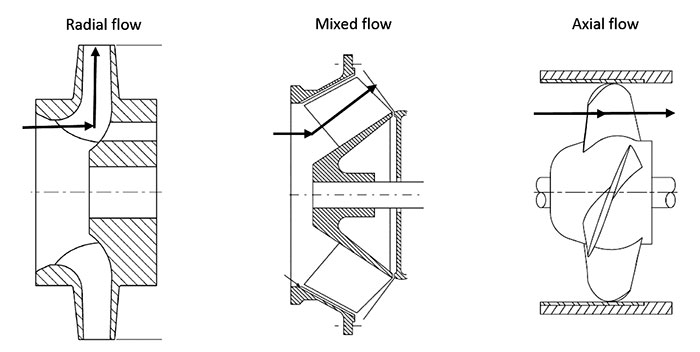
\includegraphics[width=12cm]{./figs/bom0.jpg}
\caption{Tipos de bombas rotodin\'amicas} 
\label{bom0}
\end{figure}

\begin{figure}[h]
\centering
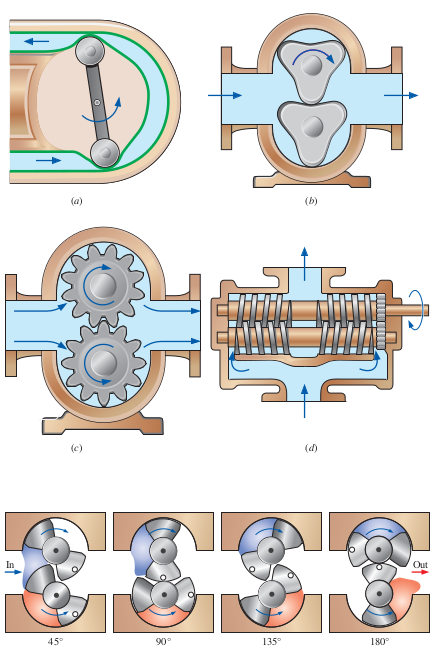
\includegraphics[width=12cm]{./figs/bom0a.png}
\caption{Tipos de bombas de desplazamiento positivo: bomba de tubo flexible, bomba de lobulo rotacional, bomba de engran\'ages y bomba de doble tornillo. } 
\label{bom0a}
\end{figure}



Las bombas mas comunes son las bombas centrifugas y centraremos la mayori\'ia de nuestro an\'alisis sobre este tipo de bombas. Una bomba centrifuga (ver figura~\ref{bom1}) esta compuesta por:

\begin{figure}[h]
\centering
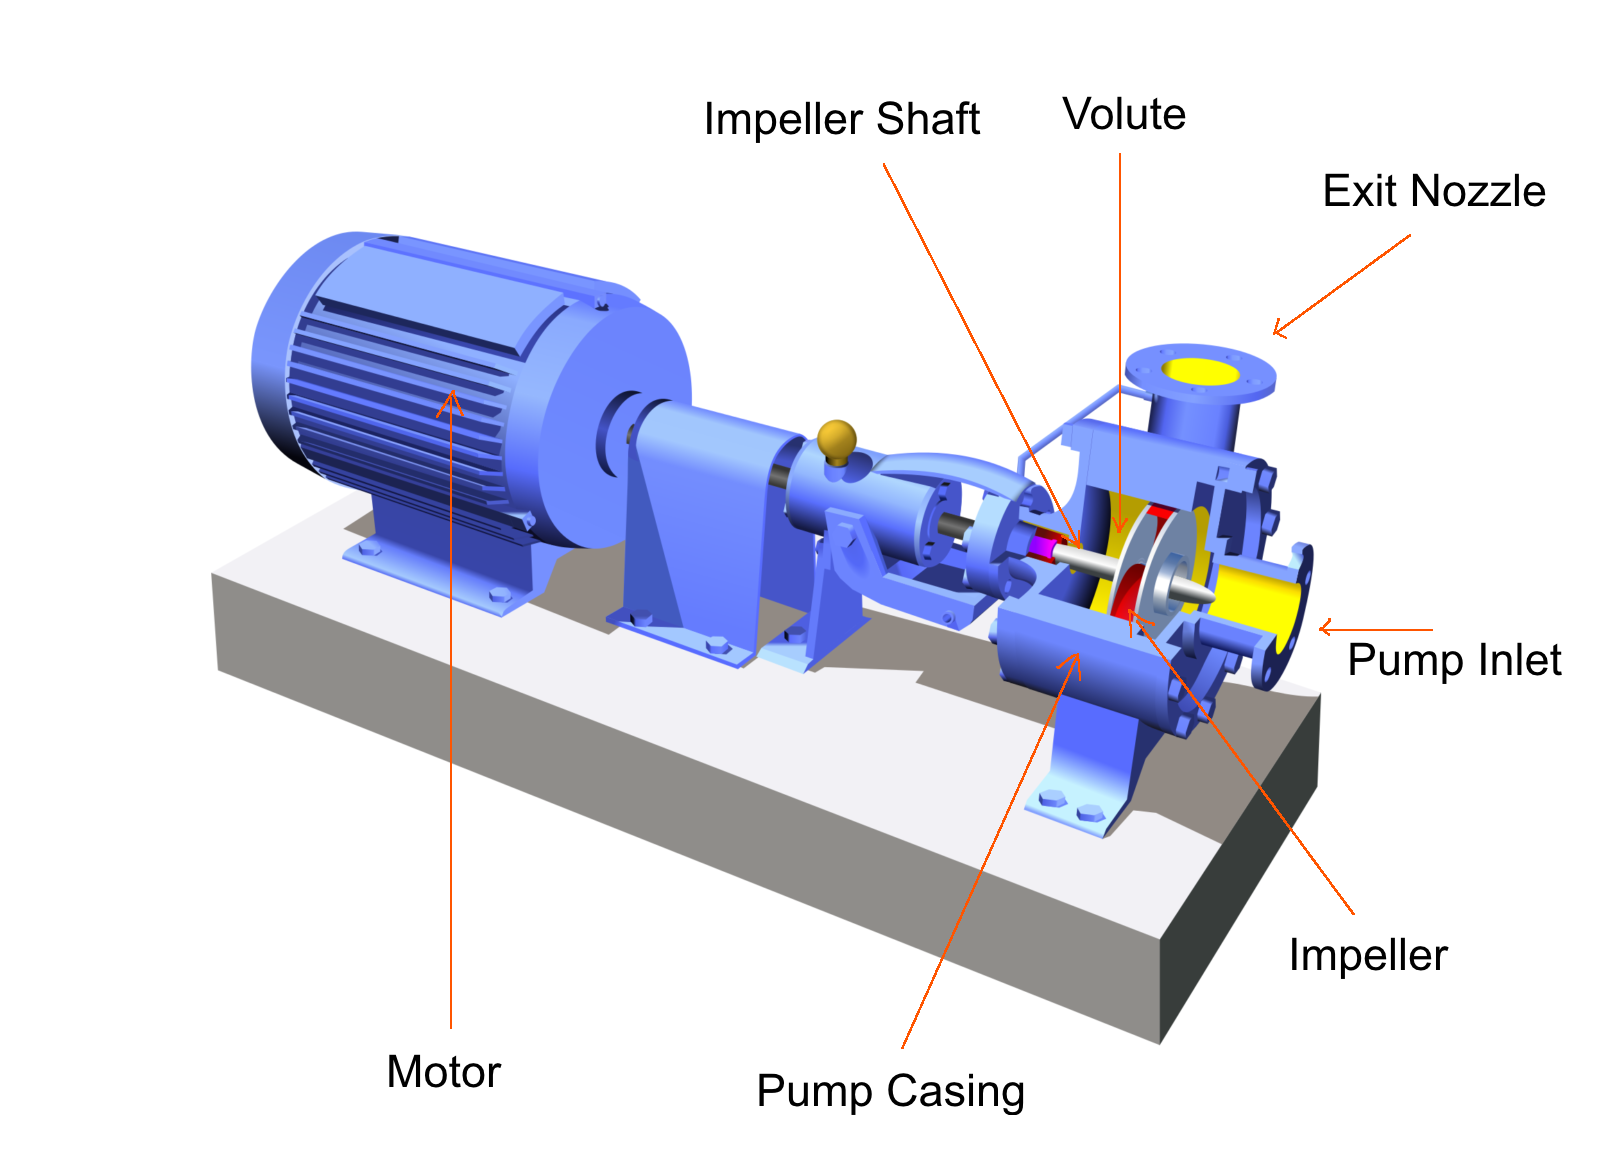
\includegraphics[width=12cm]{./figs/bom1.png}
\caption{Bombas centrifugas.} 
\label{bom1}
\end{figure}

\begin{enumerate}
\item Impulsor o rotor: Es un elemento rotatorio compuesto por \emph{alabes} que gira con una alta velocidad angular gracias al trabajo del \emph{motor}. Los alabes crean canales divergentes a trav\'es de los cuales fluye el l\'iquido.
\item Carcasa: Estructura en donde se encuentra el impulsor. Esta estructura posse un orificio por donde ingresa el fluido a baja pres\'ion (\emph{tuber\'ia de succi\'on}) y y otro por donde converge el liquido a trav\'es de los alabes y luego hacia el espiral en donde el l\'iquido es conducido hacia la tuber\'ia \emph{tuber\'ia de descarga} con una mayor presi\'on. 
\item Eje o flecha: Estructura que transfiere la potencia del motor al impulsor. 
\end{enumerate}

%%%%%%%%
\section{Ecuaciones para bombas centrifugas}
Se puede establecer ecuaciones para el calculo de potencia y de cabeza hidr\'aulica introducida por la bomba a la tuber\'ia. Cuando el flujo entra a trav\'es de la tuber\'ia de succi\'on al impulsor, este llega con una presi\'on relativamente baja, al entrar a los alabes, la velocidad angular $\omega$ con la cual se mueven los alabes, le suministra una energ\'ia al flujo el cual es expulsado (punto $S$) hacia la espiral (dentro de la carcasa) con una mayor energ\'ia (presi\'on). Teniendo en cuenta que es el impulsor el que le suministra la energ\'ia al flujo, este puede considerarse como el volumen de control para el siquiente an\'alisis. Para el an\'alisis se debe considerar lo siguiente:
\begin{itemize} 
\item flujo permanente e incompresible.
\item fricci\'on despreciable.
\item infinito n\'umero de alabes de espesor infinitesimal en el impulsor. 
\item La potencia transmitida por el eje al impulsor, es transmitida al flujo en su totalidad.
\end{itemize} 

% Cengel f14.33
\begin{figure}[h]
\centering
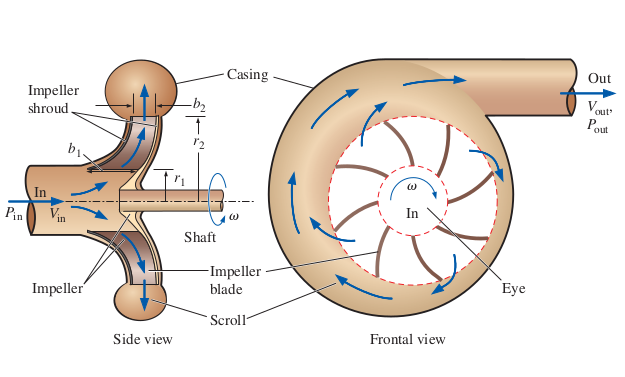
\includegraphics[width=12cm]{./figs/bom1a.png}
\caption{Impulsor y carcasa de una bomba centrifuga (tomado de \cite{cengel2013ebook}).} 
\label{bom2}
\end{figure}


% Duarte f7.3
\begin{figure}[h]
\centering
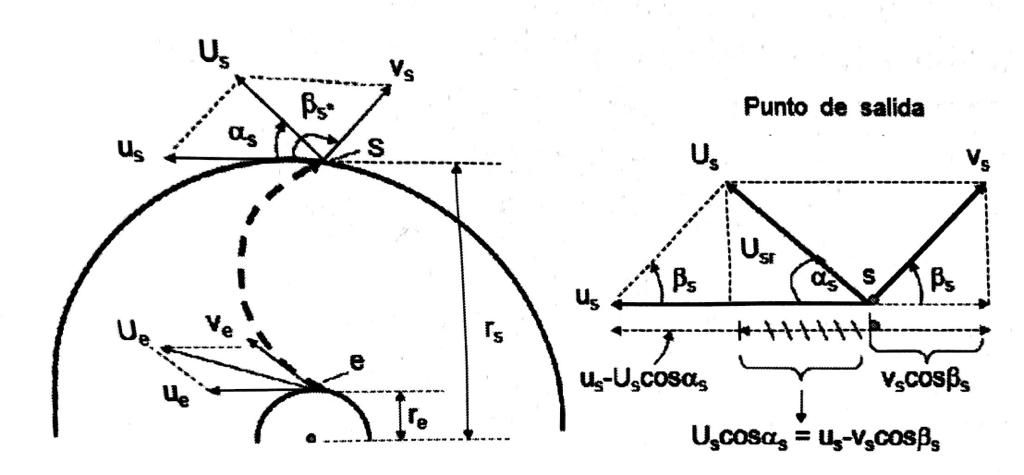
\includegraphics[width=12cm]{./figs/bom2.jpeg}
\caption{Diagramas de velocidad en el impulsor (tomado de \cite{agudelo2011mecanica}).} 
\label{bom2}
\end{figure}

Analizando el movimiento del flujo en el impulsor, este se desplaza desde el punto $e$ al punto $s$. La figura~\ref{bom2} muestra los diagramas de los vectores de velocidad en donde $U$ es la velocidad absoluta del fluido, $u$ es la velocidad tangencial en un punto en la perisfer\'ia, $v$ es la velocidad relativa del l\'iquido respecto al impulsor y tangente al alabe, $r$ es el radio del impulsor, $\alpha$ es el angulo formado por el vector de velocidad absoluta y el vector de velocidad tangente, $\beta$ es el angulo del alabe, $\beta'$ es el angulo suplementario de $\beta$, $b$ espesor del impulsor, $s$ punto de salida del flujo y $e$ es el punto de entrada del flujo. Aplicando el principio de conservaci\'on de cantidad de movimiento angular al volumen de control:

\begin{equation}
\sum M_{ext} = \frac{\gamma}{g} Q \left[ \left( \vec{r} \times \vec{U}\right)_{s} -  \left( \vec{r} \times \vec{U}\right)_{e} \right]
\label{bome1}
\end{equation}

donde $\sum M_{ext}$ es la sumatoria de los momento externos al volumen de control; el \'unico momento externo es el par de torsi\'on $T_T$ transmitido al impulsor por el eje. Los vectores posici\'on $\vec{r}$ equivalen en este caso a los radios de entrada $r_e$ y de salida $r_s$ en el impulsor. 

Analizando el diagrama de vectores de la figura~\ref{bom2}, la ecuaci\'on~\ref{bome1} se transforma en:

\begin{equation}
\color{red}\boxed{\color{black} T_T = \frac{\gamma}{g} Q \left[ \left( r U \cos \alpha \right)_{s} -  \left(r U \cos \alpha  \right)_{e} \right] }
\label{bome2}
\end{equation}

La ecuaci\'on~\ref{bome2} permite calcular el par de torsi\'on teorico transmitido por el eje al impulsor. Multiplicando la ecuaci\'on~\ref{bome2} por la velocidad angular $\omega$, se obtiene la potencia mec\'anica te\'orica:

\begin{equation}
P_T = T_T \omega = \frac{\gamma}{g} Q \left[ \left( r \omega U \cos \alpha \right)_{s} -  \left(r \omega U  \cos \alpha  \right)_{e} \right]
\label{bome3}
\end{equation}

donde $r\omega$ es la velocidad tangencial $u$. Reemplazando en la ecuaci\'on anterior:

\begin{equation}
\color{red}\boxed{\color{black} P_T =  \frac{\gamma}{g} Q \left[ \left( u U \cos \alpha \right)_{s} -  \left( u U \cos \alpha  \right)_{e} \right] }
\label{bome4}
\end{equation}

Teniendo en cuenta que no se consideran p\'erdidas en el sistema, la potencia mec\'anica te\'orica debe ser igual a la potencia hidr\'aulica te\'orica $P_H = \gamma Q h_b$ ($P_T = P_H$). Teniendo en cuenta esto, la ecuaci\'on~\ref{bome4}, queda:

\begin{equation}
 \frac{\gamma}{g} Q \left[ \left( u U \cos \alpha \right)_{s} -  \left( u U \cos \alpha  \right)_{e} \right] = \gamma Q h_b
\label{bome5}
\end{equation}

simplificando y despejando para $h_b$, se tiene:

\begin{equation}
\color{red}\boxed{\color{black} h_b= \frac{1}{g}  \left[ \left( u U \cos \alpha \right)_{s} -  \left( u U \cos \alpha  \right)_{e} \right] }
\label{bome6}
\end{equation}

Las ecuaciones~\ref{bome2}, ~\ref{bome4} y ~\ref{bome6} se conocen como las \emph{ecuaciones de Euler} para el c\'alculo del par de torsi\'on, de la potencia y de la cabeza te\'orica de una bomba centrifuga. De estas ecuaciones, es interesante anotar que mientras  la pontecia ($P_T$) y el par de torsi\'on ($T_T$) te\'oricos en este tipo de bombas depende del tipo de fluido ($\gamma$ en las ecuaciones), la cabeza ($h_b$) es independiente del fluido.

Teniendo en cuenta que los impulsores se dise\~nan de manera \'optima, el t\'ermino en la ecuaci\'on~\ref{bome6} $\left( u U \cos \alpha  \right)_{e}$ debe ser igual a cero con el fin de que $h_b$ no se disminuya en dicha cantidad. Para lograr esto, es necesario que $\cos \alpha_e$ sea igual a cero, lo cual se logra si $\alpha_e = 90^o$. Esto se logra si el vector $U_e$ forma un angulo de 90$^o$ con la horizontal logrando que no exista momento de remolino a la entrada del impulsor. Para un dise\~no \'optimo del impulsor, la ecuaci\'on~\ref{bome6} se convierte en:

\begin{equation}
 h_b= \frac{1}{g}  \left( u_s U_s \cos \alpha_s \right) 
\label{bome7}
\end{equation}

De acuerdo al diagrama de vectores de la figura\~ref{bom2}, la ecuaci\'on~\ref{bome7} se puede escribir tambi\'en como:

\begin{equation}
 h_b= \frac{1}{g}  \left[ u_s \left(u_s - v_s \cos \beta_s \right) \right] 
\label{bome8}
\end{equation}

Teniendo en cuenta que el caudal que sale del impulsor lo hace de forma radial, para luego ser canalizado por la espiral en la carcasa y dirigido hacia la tuber\'ia de descarga, dicho caudal se puede expresar como $Q = U_{rs}A_{Ls}$, donde $U_{rs}$ es la componente radial de $U$ en $s$ y $A_{Ls}$ es el \'area lateral del impulsor en la salida. De acuerdo con esto, $Q$ se puede expresar como:

\begin{equation}
Q = U_{rs} 2\pi r_s b_s
\label{bome9}
\end{equation}

donde $b_s$ es el espesor del impulsor a la salida. De la figura~\ref{bom2}, se puede demostrar que $U_{rs} = v_s \cos \beta_s \tan \beta_s$. Reemplazando en la ecuaci\'on anterior y despejando para $v_s \cos \beta_s$, se tiene:

\begin{equation}
v_s \cos \beta_s =\frac{Q}{2\pi r_s b_s \tan \beta_s}
\label{bome10}
\end{equation}

Reemplazando la ecuaci\'on~\ref{bome10} en la ecuaci\'on~\ref{bome8}, queda una expresi\'on de $h_b$ en funci\'on de $Q$ como:

\begin{equation}
\color{red}\boxed{\color{black} h_b = \frac{u_s^2}{g}- \left( \frac{u_s Q}{2\pi g r_s b_s \tan \beta_s}\right) }
\label{bome11}
\end{equation}

La ecuaci\'on~\ref{bome11} tiene la forma de una ecuaci\'on lineal $h_b = f(Q) = A-BQ$, donde A y B son constantes. Note que la ecuaci\'on~\ref{bome11} representa una familia de rectas que se denominan la \emph{curva caracter\'istica de la bomba}. Note que la ecuaci\'on~\ref{bome11} depende de $\beta_s$ por lo tanto la familia de curvas tiene el comportamiento mostrado en la figura~\ref{bom3}. El mejor comportamiento de la bomba se da cuando $0<\beta_s<90$ (alabe tirado hacia atr\'as) ya que la carga de la bomba aumenta en la medida que disminuya el caudal. 

 % Duarte f7.4
\begin{figure}[h]
\centering
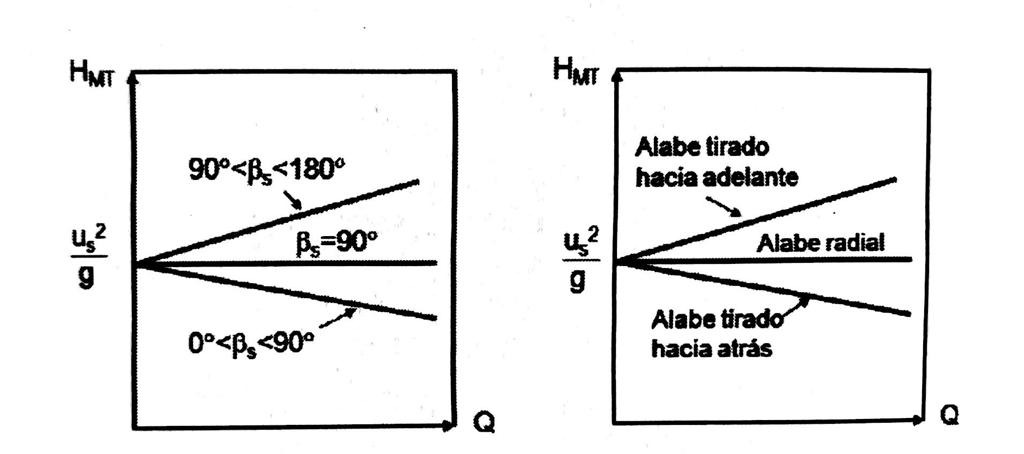
\includegraphics[width=12cm]{./figs/bom3.jpeg}
\caption{Familia de curvas caracter\'isticas te\'oricas para diferentes rangos de $\beta_s$ (tomado de \cite{agudelo2011mecanica}).} 
\label{bom3}
\end{figure}

%%%%%%%%
\section{Curva caracter\'istica real de una bomba}
Las deducciones de las ecuaciones en la secci\'on anterior se hicieron bajo supuestos te\'oricos que en la pr\'actica no obedecen a la comportamiento real de una bomba si se tiene en cuenta lo siguiente:
\begin{itemize} 
\item El n\'umero de alabes en el impulsor es finito y el espesor de cada uno de estos es diferente de cero. Esto resulta en que los alabes no son una guia perfecta para transportar el flujo (flujo circulatorio) lo que resulta en valores menores de $\beta_s$ y por lo tanto en menores valores de la componente $U_s \cos \alpha_s$. Esto significa que la carga real es menor a la te\'orica definida en la ecuaci\'on~\ref{bome11}. Esto quiere decir que la curva caracter\'istica te\'orica sufre un abatimiento tal y como se muestra en la figura~\ref{bom4}.
\item Teniendo en cuenta que existe fricci\'on debido a la rugosidad en el impulsor y que se presenta turbulencia a la salida del impulsor, dichos aspectos generan una disipaci\'on de energ\'ia que es proporcional a $Q^2$. Esto quiere decir que $h_b$ disminuye a\'un m\'as cuando $Q$ aumenta. 
\end{itemize} 
Lo anterior quiere decir que la curva caracter\'istica real presenta un comportamiento no lineal ($h_b= A-B Q^C$) similar al mostrado en la figura~\ref{bom4}.

% Duarte f7.5
\begin{figure}[h]
\centering
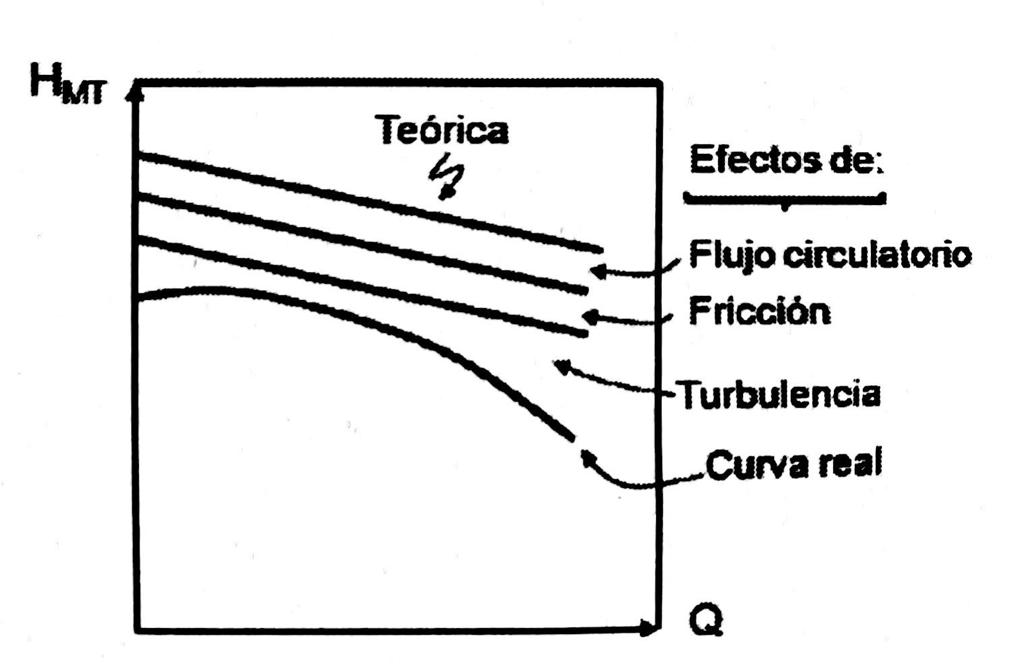
\includegraphics[width=12cm]{./figs/bom4.jpeg}
\caption{Curva caracter\'istica real (tomado de \cite{agudelo2011mecanica}).} 
\label{bom4}
\end{figure}

En las tuber\'ias de succi\'on (entrada a la bomba) donde la presi\'on suele ser baja y en la tuber\'ia de descarga (salida de la bomba) en donde la presi\'on es alta, es com\'un instalar man\'ometros o sensores para determinar la presi\'on en estos dos puntos. Aplicando la ecuaci\'on de Bernoulli entre la ubicaci\'on de estos dos man\'ometros, se puede determinar la cabeza \'util del flujo:


\begin{equation}
h_m = \left(\frac{p}{\gamma} + \frac{V^2}{2g} + z \right)_{sc} - \left(\frac{p}{\gamma} + \frac{V^2}{2g} + z \right)_{d} + h_e
\label{bome12}
\end{equation}

donde los subindices $sc$ indican tuber\'ia de succi\'on y $d$ tuber\'ia de descarga. De acuerdo con la ecuaci\'on~\ref{bome12}, la potencia se expresa como $P_u = \gamma Q h_m$. La eficiencia de una bomba definida por el dise\~no de los alabes, de la carcasa y de las condiciones de operac\'on, se puede determinar como la relaci\'on de la potencia \'util ($P_u$) y la potencia que aplica el motor a la bomba ($P_T$):

\begin{equation}
\eta_b = \frac{P_u}{P_T} = \frac{\gamma Q h_m}{T_T \omega}
\label{bome13}
\end{equation}

donde $T_T$ es el torque te\'orico (ver ecuaci\'on~\ref{bome3}). La eficiencia del motor se puede definir como la potencia que aplica el motor a la bomba ($P_T$) y la potencia de salida del motor (o \emph{potencia al freno}, bhp) ($P_m$):

\begin{equation}
\eta_m = \frac{P_T}{P_m} = \frac{T_T \omega}{P_m}
\label{bome14}
\end{equation}

La eficiencia global de todo el sistema (motor, flecha y bomba) queda definida como:

\begin{equation}
\eta =\eta_b \eta_m = \frac{\gamma Q h_m}{P_m}
\label{bome15}
\end{equation}

Se pueden definir otras curvas caracter\'isticas como potencia al freno o potencia de salida del motor $P_m$ vs $Q$ o eficiencia de la bomba $\eta_b$ vs $Q$ como se muestra en la figura~\ref{bom5}. 

% Duarte f7.6
\begin{figure}[h]
\centering
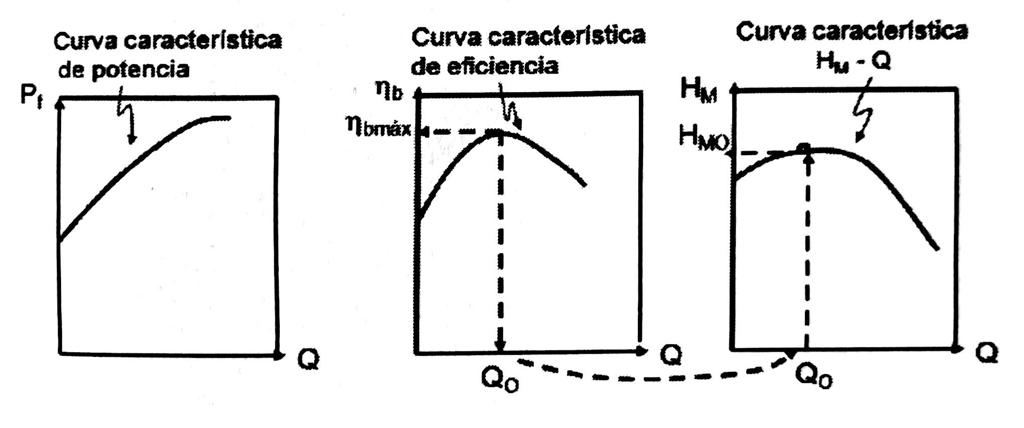
\includegraphics[width=12cm]{./figs/bom5.jpeg}
\caption{Otras curvas caracter\'isticas (tomado de \cite{agudelo2011mecanica}).} 
\label{bom5}
\end{figure}

N\'otese que en la figura~\ref{bom5}, $P_m$ aumenta a medida que $Q$ aumenta, mientras que la eficiencia de la bomba $\eta_b$ aumenta hasta alcanzar un m\'aximo y luego disminuye. Este punto de m\'axima eficiencia define el caudal ($Q_o$) con el cual deber\'ia operar la bomba, lo cual se da rara vez. 

% Cengel f14.8
\begin{figure}[h]
\centering
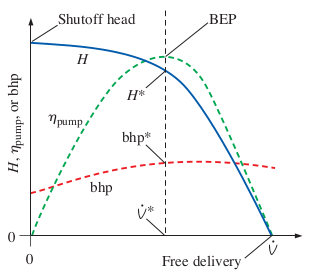
\includegraphics[width=12cm]{./figs/bom5a.png}
\caption{Curvas caracter\'isticas y best efficiencie point (BEP) para una bomba centrifuga (tomado de \cite{cengel2013ebook}).} 
\label{bom5a}
\end{figure}

% Cengel f14.9
\begin{figure}[h]
\centering
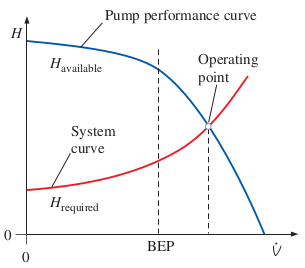
\includegraphics[width=12cm]{./figs/bom5b.png}
\caption{Punto de operaci\'on (caudal) de la bomba para un sistema de tuber\'ias (tomado de \cite{cengel2013ebook}).} 
\label{bom5b}
\end{figure}

En la practica, estas curvas caracter\'isticas son construidas por el fabricante de la bomba en laboratorios de hidr\'aulica  equipados con instrumentos de alta presici\'on. Lo m\'as com\'un es encontrar las curvas para una velocidad constante de rotaci\'on de la flecha de la bomba y para diferentes di\'ametros del impulsor (ver figura~\ref{bom6}). Tambi\'en es com\'un encontrar las curvas caracter\'isticas de la bomba para un impulsor variando la velocidad de rotaci\'on (ver figura~\ref{bom7}). Estas curvas que son presentadas por el fabricante en manuales, se pueden construir para diferentes tipos de bombas usando \emph{an\'alisis dimensional}. Es posible encontrar curvas caracter\'isticas de $h_m$ vs $Q$ para diferentes bombas (diferentes di\'ametros del impulsor) representadas en el mismo sistema de referencia, con el fin seleccionar m\'as de una bomba para valor de $Q_o$. Esto se hace con el fin de determinar la mejor opci\'on entre las posible bombas con base en an\'alisis de costos de operaci\'on de estas.    

% Duarte f7.10
\begin{figure}[h]
\centering
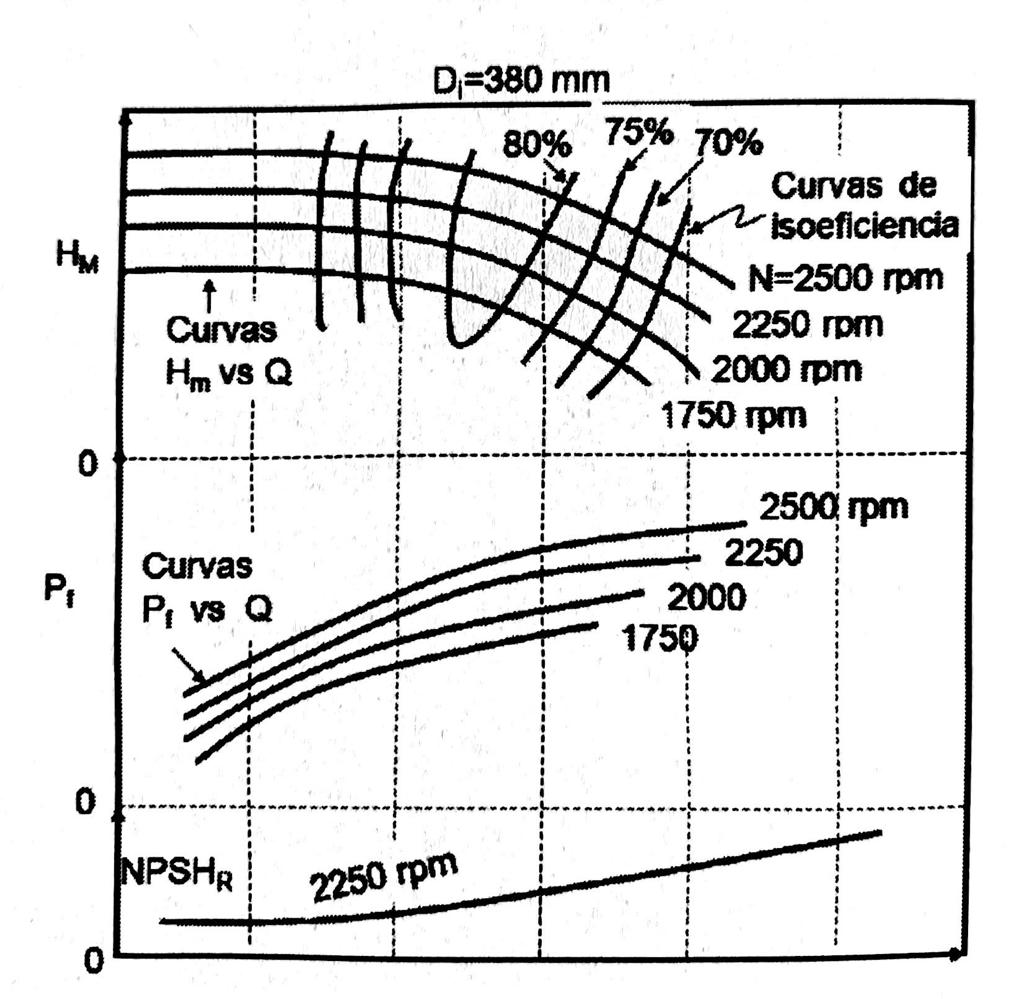
\includegraphics[width=12cm]{./figs/bom7.jpeg}
\caption{Curva caracter\'istica para $D$ (di\'ametro externo del impulsor) constante (tomado de \cite{agudelo2011mecanica}).} 
\label{bom7}
\end{figure}


% Cengel f14.9
\begin{figure}[h]
\centering
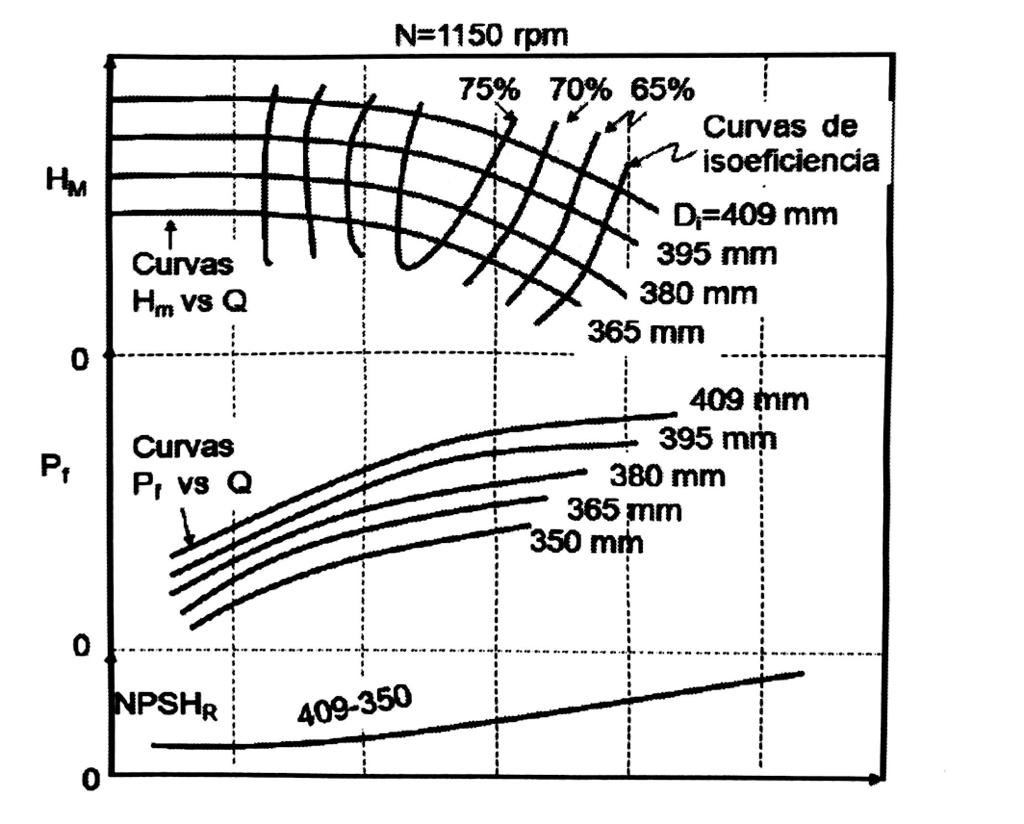
\includegraphics[width=12cm]{./figs/bom6.jpeg}
\caption{Curva caracter\'istica para $\omega$ constante (tomado de \cite{agudelo2011mecanica}).} 
\label{bom6}
\end{figure}

%%%%%%%
\section{Analisis dimensional en bombas centrifugas}
En la secci\'on anterior se coment\'o que los fabricantes de bombas poseen cartillas en donde se incluyen los diferentes tipos de curvas caracter\'isticas de las bombas que fabrican (ver figuras~\ref{bom6} y ~\ref{bom7}). Estas curvas se utilizan  para escoger la mejor opci\'on de acuerdo con las necesidades del usuario. Para la construcci\'on de estas curvas caracter\'isticas se construyen modelos en el laboratorio que sean geom\'etricamente similares al prototipo, en particular el impulsor.

En el an\'alisis de bombas centrifugas, las variables que intervienen son las siguientes: carga o cabeza \'util $h_m$ [$L$], caudal $Q$ [$L^3 T^{-1}$], velocidad de rotaci\'on en rpm $\omega$ [$T^{-1}$], di\'ametro del impulsor $D_i$ [$L$], viscosidad cinem\'atica $\nu$ [$L^2 T^{-1}$], aceleraci\'on de la gravedad $g$ [$L T^{-2}$]. En total se tienen 6 variables y 2 dimensiones ($L$ y $T$), lo cual quiere decir que el n\'umero de par\'ametros adimencionales que se pueden formar a partir de las variables es 4 (6-2=4). Se deben definir dos  (debido a que son dos dimensiones involucradas) variables repetitivas, las cuales deben ser independientes entre si; estas varibles son $\omega$ y $D_i$. Haciendo an\'alisis dimensional para la funci\'on $f(h_m, Q, \omega, D_i, g, \nu)$, se tienen los siguientes parametros:

\begin{equation}
\Pi_1 = \frac{h_m}{D_i} \quad  \Pi_2 = \frac{Q}{\omega D_i^3} \quad \Pi_3 = \frac{g}{\omega^2 D_i} \quad \Pi_4 = \frac{\omega D_i^2}{\nu}
\label{boma1}
\end{equation}

Como la intenci\'on del analisis dimensional es tener una funci\'on $h_m = f(Q)$ (curva caracter\'istica), se tiene:

\begin{equation}
\Pi_1 =f\left(\Pi_2, \Pi_3, \Pi_4 \right) 
\label{boma2}
\end{equation}

Reemplanzando en la ecuaci\'on~\ref{boma2}, tenemos:

\begin{equation}
\frac{h_m}{D_i} = f\left( \frac{Q}{\omega D_i^3}, \frac{g}{\omega^2 D_i} , \frac{\omega D_i^2}{\nu} \right)
\label{boma3}
\end{equation}

Teniendo en cuenta que se debe satisfacer una similitud geom\'etrica entre el modelo y el prototipo, se hace imposible tener el mismo n\'umero de Reynolds (parametro $\Pi_4$) en el modelo y en el prototipo, lo cual hace necesario despreciar los efectos de la viscosidad. Por otro lado, gracias a la experimentaci\'on se ha demostrado que $\Pi_1 = f(\Pi_3^{-1})$. De acuerdo con esto:

\begin{equation}
\frac{h_m}{D_i} = \frac{\omega^2 D_i}{g} f\left( \frac{Q}{\omega D_i^3}   \right)
\label{boma4}
\end{equation}

Agrupando en la ecuaci\'on~\ref{boma4}, se tiene:

\begin{equation}
\frac{g h_m}{\omega^2 D_i^2} = f\left( \frac{Q}{\omega D_i^3}   \right)
\label{boma5}
\end{equation}

En el lado izquierdo de la ecuaci\'on~\ref{bom5} se forma otro  par\'ametro adimensional($\Pi_5$), por lo que la ecuaci\'on se puede expresar como $\Pi_5 = f(\Pi_2)$. En la ecuaci\'on~\ref{boma5} $\Pi_2$ se denomina el \emph{par\'ametro de caudal} y el $\Pi_5$ es le \emph{par\'ametro de carga o cabeza}. La ecuaci\'on~\ref{boma4} es la  \emph{curva caracter\'istica adimensional} de la bomba y es la misma para una \emph{serie hom\'olaga} de bombas. Dicha serie homologa implica una similaridad geom\'etrica entre bombas, es decir, que sus  diagramas vectoriales en el impulsor sean semejantes y que sus eficiencias sean las mismas. Del an\'alisis dimensional, es posible formar un un tercer par\'ametro adimensional como el producto entre $\Pi_5$ y $\Pi_2$, dicho p\'arametro adimensional ($\Pi_6$) es conocido como el \emph{par\'ametro de potencia}:

\begin{equation}
\Pi_6 = \frac{P_m}{\rho \omega^3 D_i^5}
\label{boma6}
\end{equation}

En una serie homologa, los par\'ametros $\Pi_5$, $\Pi_2$ y $\Pi_6$ son constantes en cada bomba de la serie. 

\subsection{Aplicaci\'on de los par\'ametros adimensionales}
\subsubsection*{Operaci\'on de la misma bomba a velocidad ($\omega$) variable}
En este caso se estudia el comportamiento de la bomba con una velocidad angular variable pero con el mismo impulsor ($D_i$ constante). Como $D_i$ es constante, los parametros adimensionales quedan expresados como:

\begin{equation}
\color{red}\boxed{\color{black} \frac{Q}{\omega} = \text{const} \quad \frac{h_m}{\omega^2}= \text{const}  \quad \frac{P_m}{\omega^3}= \text{const} }
\label{boma7}
\end{equation}

De las relaciones anteriores, se tiene que $h_m \propto Q^2$, ecuaci\'on que representa una par\'abola en donde todos sus puntos indican igual similitud (la misma eficiencia). Si se tiene la idea de que se ha obtenido una curva caracter\'istica ($h_m$ vs$Q$) del modelo de una bomba dentro de una serie homologa para una velocidad angular $\omega_A$, a partir de esta curva es posible obtener la curva de la misma bomba pero operando a una velocidad angular $\omega_B$ bajo condiciones din\'amicas de flujo similares (ver figura~\ref{bom8}). Aplicando las leyes de similitud para puntos sobre una misma curva de isoeficiencia, por ejemplo los puntos 1 y 2, para la curva $\omega_A$ y para la curva $\omega_B$ respectivamente, en donde se conocen $h_{m_1}$, $Q_1$ y $\nu_1 = \nu_2$, se pueden encontrar los valores de $Q_2$ y $h_{m_2}$ de la siguiente manera:

% Duarte f7.15
\begin{figure}[h]
\centering
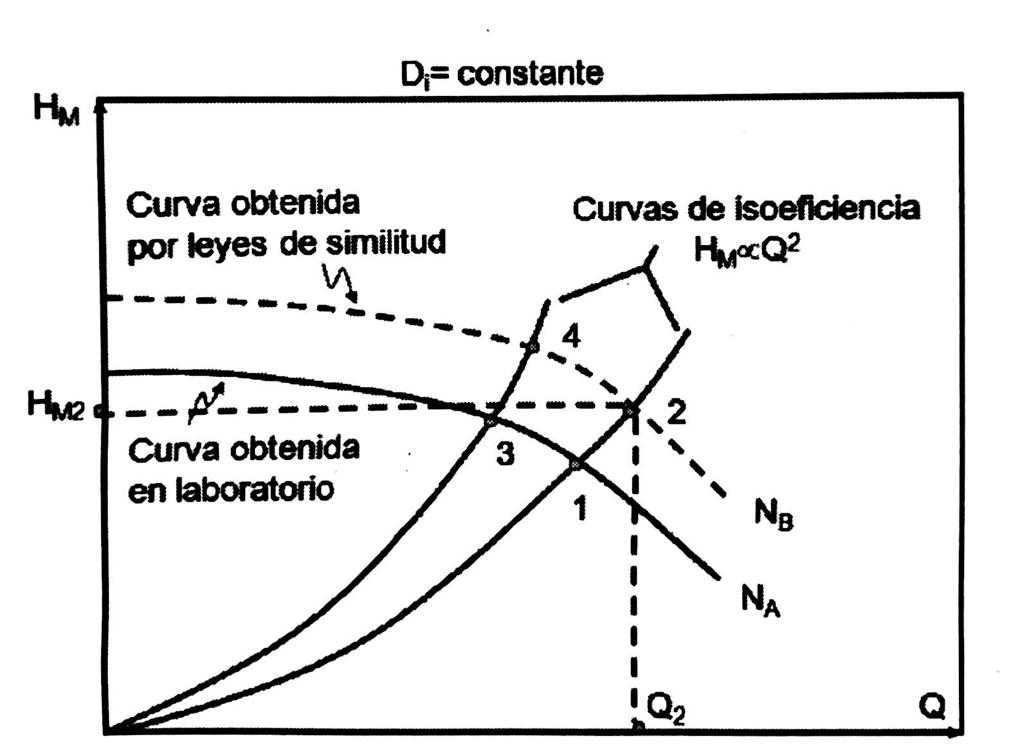
\includegraphics[width=12cm]{./figs/bom8.jpeg}
\caption{Obtenci\'on de curvas caracter\'isticas usando an\'alisis dimensional para un $D_i$ (tomado de \cite{agudelo2011mecanica}).} 
\label{bom8}
\end{figure}


\begin{equation}
\Pi_{2_1} = \Pi_{2_2} \quad \left( \frac{Q}{\omega D_i^3} \right)_{2_1} = \left( \frac{Q}{\omega D_i^3} \right)_{2_2} \quad Q_2 = Q_1 \frac{\omega_B}{\omega_A}
\label{boma8}
\end{equation}

\begin{equation}
\Pi_{5_1} = \Pi_{5_2} \quad \left( \frac{h_m}{\omega^2 D_i^2} \right)_{5_1} = \left( \frac{h_m}{\omega^2 D_i^2} \right)_{5_1} \quad h_{m_2} = h_{m_1} \left(\frac{\omega_B}{\omega_A}\right)^2
\label{boma9}
\end{equation}


Analizando la figura~\ref{bom8}, cuando $\omega_A < \omega_B$, el punto 2 (de la nueva curva caracter\'istica) se ubicar\'a arriba y a la derecha del punto 1. Si $\omega_A > \omega_B$, el punto 2 se ubicar\'a abajo y a la izquierda del punto 1. Si se desea obtener otro punto, por ejemplo el punto 4, sobre la nueva curva caracter\'istica para $\omega_B$, se escoge el punto 3 en la curva de $\omega_A$ y se aplica el procedimiento descrito en las ecuaciones~\ref{boma8} y ~\ref{boma9} para encontrar $Q_4$ y $h_{m_4}$. De la misma manera se pueden escoger otros puntos sobre la curva de $\omega_A$ para ir encontrado la curva de $\omega_B$. De igual manera, se pueden encontrar las curvas caracter\'isticas para otros valores de $\omega$.


\subsubsection*{Operaci\'on de la misma bomba con diferentes impulsores ($D_i$)}
Si se opera la misma bomba con la misma velocidad $\omega$ pero con diferentes tama\~nos ($D_i$) de los impulsores, es posible obtener las curvas caracter\'isticas para diferentes valores de $D_i$. Sin embargo, debido a que el impulsor cambia, la similitud geom\'etrica no se cumple. Gracias a la experiencia se ha podido establecer que para $\omega$ constante:

\begin{equation}
\color{red}\boxed{\color{black} \frac{Q}{D_i} = \text{const} \quad \frac{h_m}{D_i^2}= \text{const}  \quad \frac{P_m}{D_i^3}= \text{const} }
\label{boma7}
\end{equation}

De la anterior ecuaci\'on se tiene que $Q \propto D_i$ y $h_m \propto D_i^2$, por lo tanto $h_m \propto Q^2$. Esta \'ultima relaci\'on representa una par\'abola donde todos los puntos tienen igual similitud (la misma eficiencia). Si se obtiene una curva caracter\'istica de $h_m$ vs $Q$ para un di\'ametro del impulsor $D_{i_A}$ con una velocidad $\omega$ gracias al trabajo experimental, es posible obtener una familia de curvas caracter\'isticas para la misma bomba pero con diferentes valores de $D_i$ a una velocidad constante $\omega$. De acuerdo con la figura~\ref{bom9}, si se conoce la curva para $D_{i_A}$ y se desea conoce la curva para $D_{i_B}$, se toma el punto 1 (sobre la curva para $D_{i_A}$) donde se conoce $h_{m_1}$, $Q_1$ y $\nu_1 = \nu_2$, y se toma el punto 2 (sobre la curva para $D_{i_B}$) y se calcula $Q_2$ y $h_{m_2}$ como:

% Duarte f7.16
\begin{figure}[h]
\centering
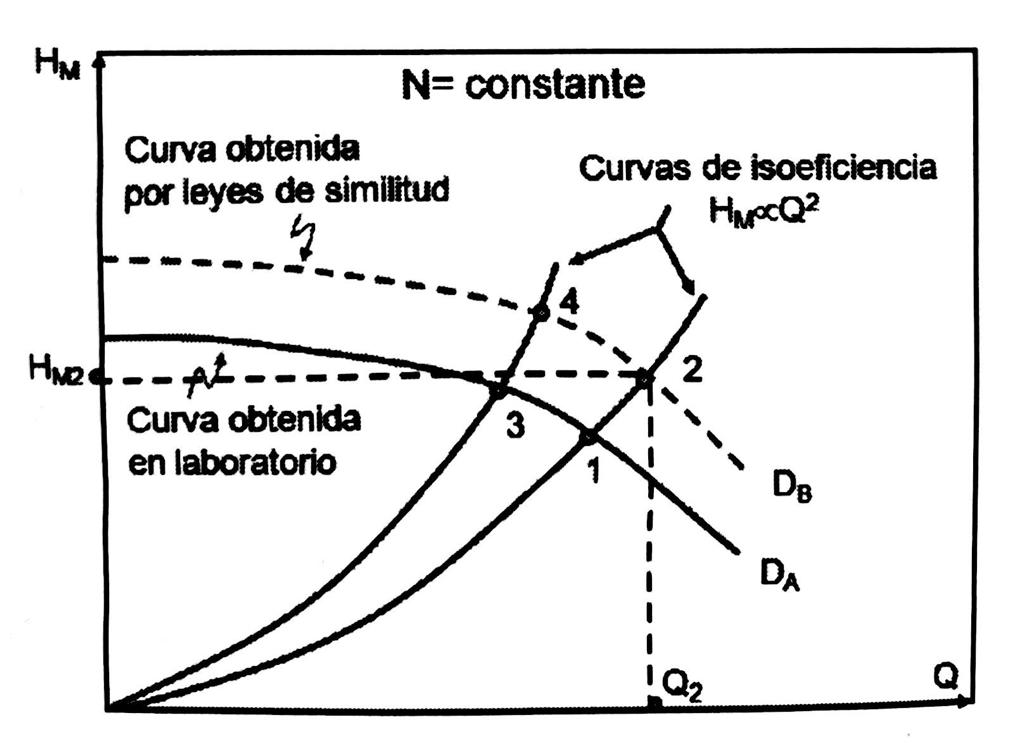
\includegraphics[width=12cm]{./figs/bom9.jpeg}
\caption{Obtenci\'on de curvas caracter\'isticas usando an\'alisis dimensional para un $\omega$ (tomado de \cite{agudelo2011mecanica}).} 
\label{bom9}
\end{figure}


\begin{equation}
\Pi_{2_1} = \Pi_{2_2} \quad \left( \frac{Q}{D_i} \right)_{2_1} = \left( \frac{Q}{D_i} \right)_{2_2} \quad Q_2 = Q_1 \frac{D_{i_B}}{D_{i_A}}
\label{boma10}
\end{equation}

\begin{equation}
\Pi_{5_1} = \Pi_{5_2} \quad \left( \frac{h_m}{D_i^2} \right)_{5_1} = \left( \frac{h_m}{D_i^2} \right)_{5_1} \quad h_{m_2} = h_{m_1} \left(\frac{D_{i_B}}{D_{i_A}}\right)^2
\label{boma11}
\end{equation}
 
Observando la figura~\ref{bom9}, cuando $D_{i_A} < D_{i_B}$, el punto 2 se encuentrar\'a arriba y a la derecha del punto 1, mientras que cuando $D_{i_A} > D_{i_B}$ el punto 2 se encontrara abajo y a la izquierda del punto 1. Otros valores de $h_m$ y $Q$ para otros puntos sobre la curva para $D_{i_B}$ se obtendr\'an utilizando las ecuaciones~\ref{boma10} y ~\ref{boma11}. 

\subsection{Velocidad espec\'ifica}
La velocidad espec\'ifica ($n_s$) de una unidad (bomba) perteneciente a una serie homologa es una cantidad muy usada en la selecci\'on y dise\~no preliminar de una bomba. Para una serie hom\'ologa se debe cumplir:
\begin{enumerate} 
\item $ \frac{Q}{\omega D_i^3} = \text{const} \quad \text{por lo que} \quad D_i \propto \left( \frac{Q}{\omega} \right)^{1/3} $
\item $ \frac{g h_m}{\omega^2 D_i^2} = \text{const} \quad \text{por lo que} \quad D \propto \left( \frac{\sqrt{g h_m}}{\omega} \right) $
\end{enumerate} 

De acuerdo con las expresiones anteriores, se puede definir una relaci\'on de mayor importancia entre $Q$ y $h_m$:

\begin{equation}
\left( \frac{Q}{\omega} \right)^{1/3} \propto \frac{\sqrt{g h_m}}{\omega} \quad \text{por lo que} \quad \frac{Q^{1/3} \omega}{\omega^{1/3} \sqrt{g h_m}} = \text{const}
\label{boma12}
\end{equation}

Elevando el numerador y el denominador de la ecuaci\'on~\ref{boma12} a la $3/2$, se tiene:

\begin{equation}
 \frac{\omega \sqrt{Q}}{ h_m^{3/4}} = \text{const}
\label{boma13}
\end{equation}

Con base en la ecuaci\'on~\ref{boma13}, la velocidad espec\'ifica de una serie de bombas homologas se define como la velocidad de una de ellas, con cierto tama\~no, tal que suministre un caudal unitario contra una carga unitaria, es decir:

\begin{equation}
\color{red}\boxed{\color{black} n_s= \frac{\omega \sqrt{Q^*} }{ h_m^{*3/4}} }
\label{boma14}
\end{equation}

donde $Q^*$ y $h_m^*$ representan el caudal y la carga para una eficiencia m\'axima del sistema (ver figura~\ref{bom11}). $n_s$ se puede interpretar como la velocidad para la cual modelos geom\'etricamente similares a prototipos de las diferentes clases de bombas operar\'ian para mover un caudal unitario (e.g. 1 gpm) cuando se genera una cabeza unitaria (e.g. 1 pie). Note que las unidades de $n_s$ no son las unidades de velocidad y si se divide la ecuaci\'on~\ref{boma14} por $g^{3/4}$, $n_s$ se convierte en un par\'ametro adimensional.

% Duarte F7.24
\begin{figure}[h]
\centering
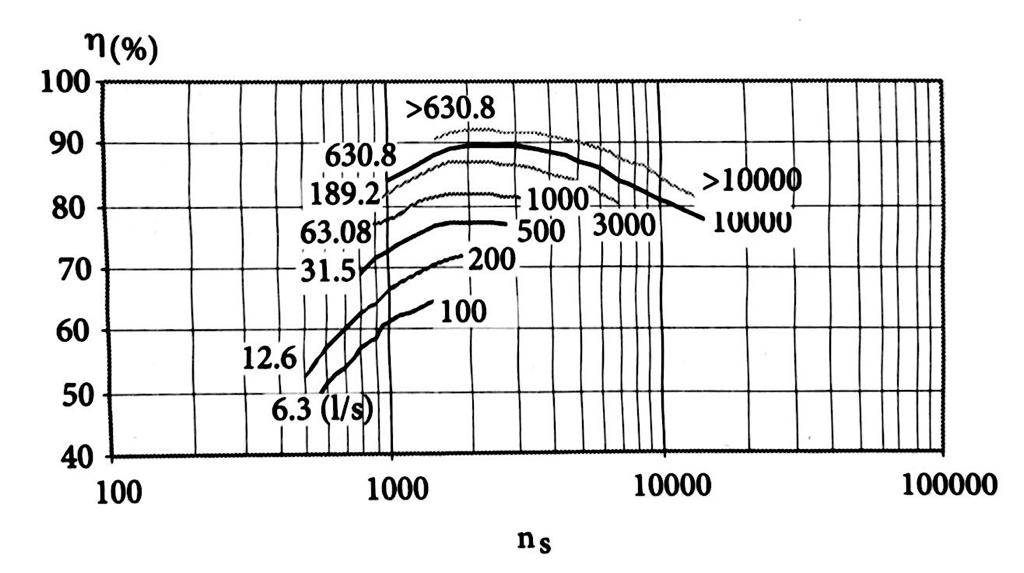
\includegraphics[width=12cm]{./figs/bom11.jpeg}
\caption{Velocidad espef\'ica ($n_s$) vs eficiencia de la bomba ($\nu_b$)  (tomado de \cite{agudelo2011mecanica}).} 
\label{bom11}
\end{figure}


De acuerdo con los valores $n_s$, las bombas rotodin\'amicas se pueden clasificar como: \emph{bombas de flujo radial}, \emph{bombas de flujo mixto} y \emph{bombas de flujo axial}.  La figura~\ref{bom10} muestra los rangos de $n_s$ para cada tipo de bomba en sistema internacional y en sistema ingles.

% Duarte T7.2
\begin{figure}[h]
\centering
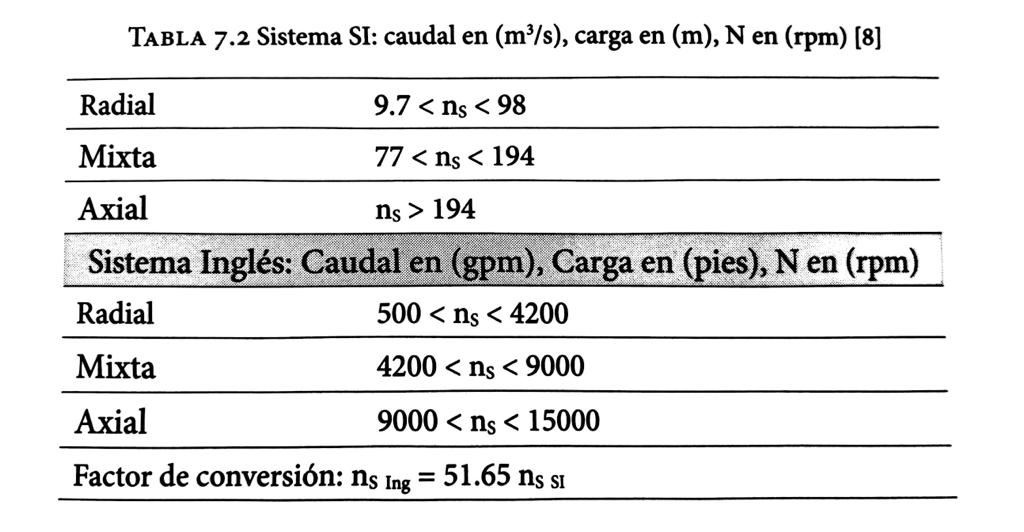
\includegraphics[width=12cm]{./figs/bom10.jpeg}
\caption{Valores de referencia de la velocidad relativa en sistema internacional y sistema ingles (tomado de \cite{agudelo2011mecanica}).} 
\label{bom10}
\end{figure}


Analizando los valores de $n_s$ en la figura~\ref{boma10} y la ecuaci\'on~\ref{boma14} se puede deducir  que las bombas radiales, por tener el rango menor para $n_s$, son \'utiles para proyectos que requieren grandes cargas y caudales peque\~nos. En contraste, las bombas de flujo axial son recomendables para proyectos con baja carga pero con altos caudales.  

Generalmente, las bombas con un solo impulsor, pueden utilizarse para una carga m\'axima de $h_m = 60$ m. Para mayores valores de $h_m$ es necesario utilizar \emph{bombas de pasos m\'ultiples} las cuales tienen varios impulsores acoplados a una misma flecha. En el caso de requerirse el bombeo de grandes caudales con baja carga, es necesario utilizar bombas de flujo axial o flujo mixto con \emph{doble succi\'on} en donde cada tuber\'ia de succi\'on esta conectada con un impulsor. 

%%%%%%%
\section{Estaciones de bombeo}
Una bomba se coloca en un sistema de tuber\'ias con el fin de a\~nadir energ\'ia al flujo para transportarlo de un punto a otro. Entre estos puntos existen diferencias topogr\'aficas y perdidas de energ\'ia que deben ser vencidas por la energ\'ia adicional suministrada por la bomba. Las bombas convierten energ\'ia mec\'anica de rotaci\'on en energ\'ia cin\'etica o de presi\'on en el fluido. Este aumento de energ\'ia es detectado por los man\'ometros, usualmente colocados, en la tuber\'ia de succi\'on y en la tuber\'ia de descarga. Esta adici\'on de energ\'ia a trav\'es de la bomba cambia las l\'ineas de gradiente hidr\'aulico y de energ\'ia. Algunas aspectos que caracterizan una estaci\'on de bombeo, son los siguientes (ver figura~\ref{bom12}):

% Duarte F8.1
\begin{figure}[h]
\centering
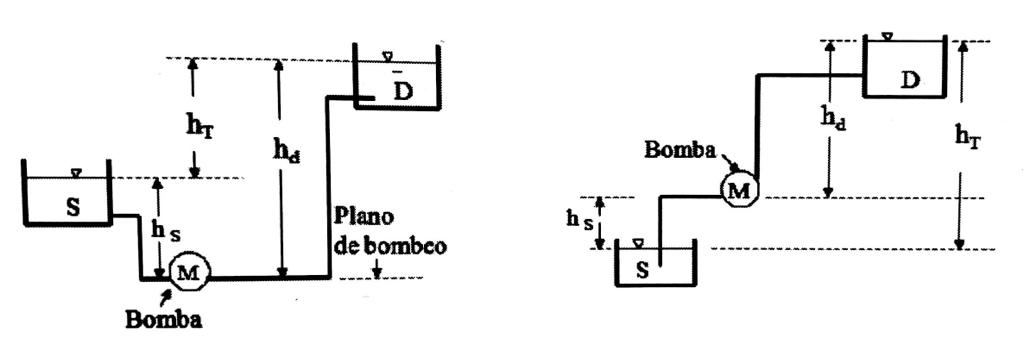
\includegraphics[width=12cm]{./figs/bom18.jpeg}
\caption{Estaciones de bombeo (tomado de \cite{agudelo2011mecanica}).} 
\label{bom12}
\end{figure}

\begin{itemize}
\item \emph{Plano de bombeo}: Es el plano horizontal en donde se ubica la bomba.  
\item \emph{Carga est\'atica de descarga ($h_d$)}: Es la distancia vertical entre el plano de bombeo y la superficie libre del deposito de descarga. 
\item \emph{Carga est\'atica de succi\'on ($h_s$)}: Es la distancia vertical desde la superficie libre del tanque de succi\'on al plano de bombeo.
\item \emph{Carga est\'atica total ($h_T$)}: Es la distancia vertical entre la superficie libre del tanque de succi\'on y la superficie libre del tanque de descarga. 
\end{itemize}

\subsection{Curva de la estaci\'on}
Si se aplica la ecuaci\'on de Bernoulli entre el tanque de succi\'on y el tanque de descarga (ver figura~\ref{bom12}), se tiene:

\begin{equation}
H_1 + h_m = H_2 + \sum h_f + \sum h_e 
\label{boma15}
\end{equation}

donde $H_1$ es la energ\'ia en la succi\'on, $H_2$ es la energ\'ia en la descarga, $h_m$ es la carga de la bomba, y la sumatoria de $h_f$ y $h_e$ son las perdidas por fricci\'on y por accesorios a lo largo de la tuber\'ia. Si decimos que $h_T = H_2-H_1$ y que las perdidas se pueden expresar en funci\'on del caudal, la ecuaci\'on~\ref{boma15} se convierte en:

\begin{equation}
h_m = h_T + (C+K)Q^2 = h_T +A Q^2
\label{boma16}
\end{equation}

donde $A$ es una constante igual a $A = \frac{fL}/{D A^2 2 g} + \frac{1}{2g A^2}\sum K$. Note que la ecuaci\'on establece una relaci\'on de la carga de la bomba, $h_m$, como una funci\'on de la carga est\'atica, $h_T$, y del caudal. Esta ecuaci\'on se denomina la \emph{curva de la estaci\'on} o la \emph{curva del sistema} y representa la energ\'ia por unidad de peso que requiere el sistema. 

Analizando la figura~\ref{bom13} se observa que la curva del sistema no inicia en el origen del sistema de coordenadas, por lo que para un caudal $Q=0$ el sistema exige una energ\'ia igual a $h_T$. La forma de la curva depende de las perdidas a lo largo del sistema. 

% Saldarriaga F4.3
\begin{figure}[h]
\centering
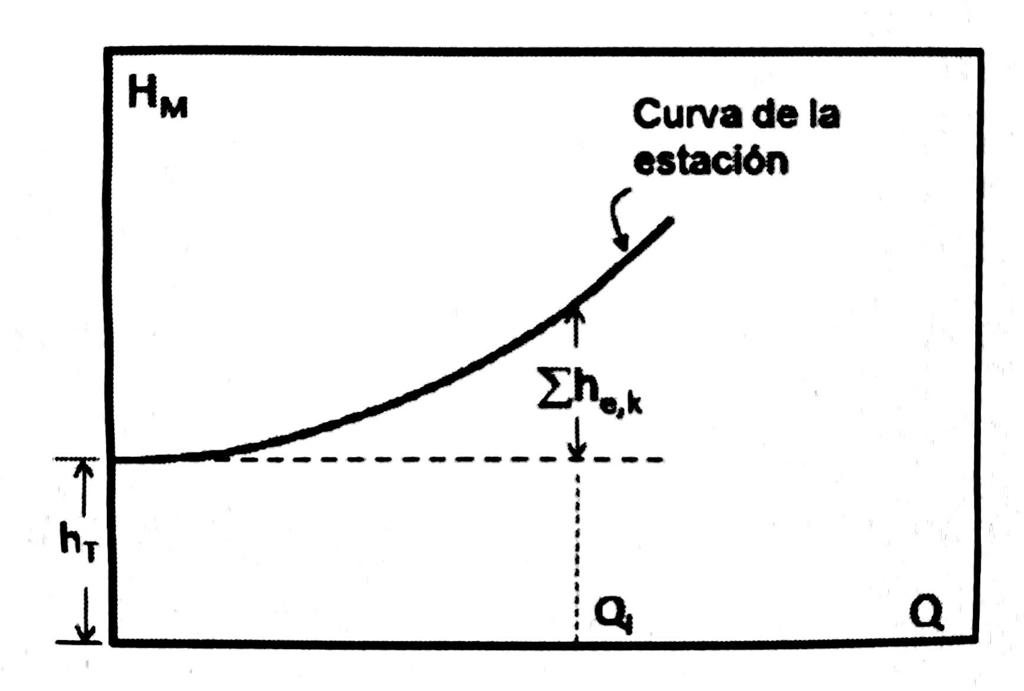
\includegraphics[width=12cm]{./figs/bom13.jpeg}
\caption{Curva de la estaci\'on en un sistema tanque-bomba-tuber\'ia (tomado de \cite{agudelo2011mecanica}).} 
\label{bom13}
\end{figure}

Dibujando la curva del sistema en el gr\'afico de curva caracter\'istica de una bomba para una velocidad $\omega$ constante y diferentes impulsores (diferentes valores de $D_i$), la intersecci\'on de la curva del sistema con las curvas caracter\'isticas genera un \emph{punto de operaci\'on} para cada impulsor ($T_1$, $T_2$, $T_3$) (ver figura~\ref{bom14}).

% Duarte F8.3
\begin{figure}[h]
\centering
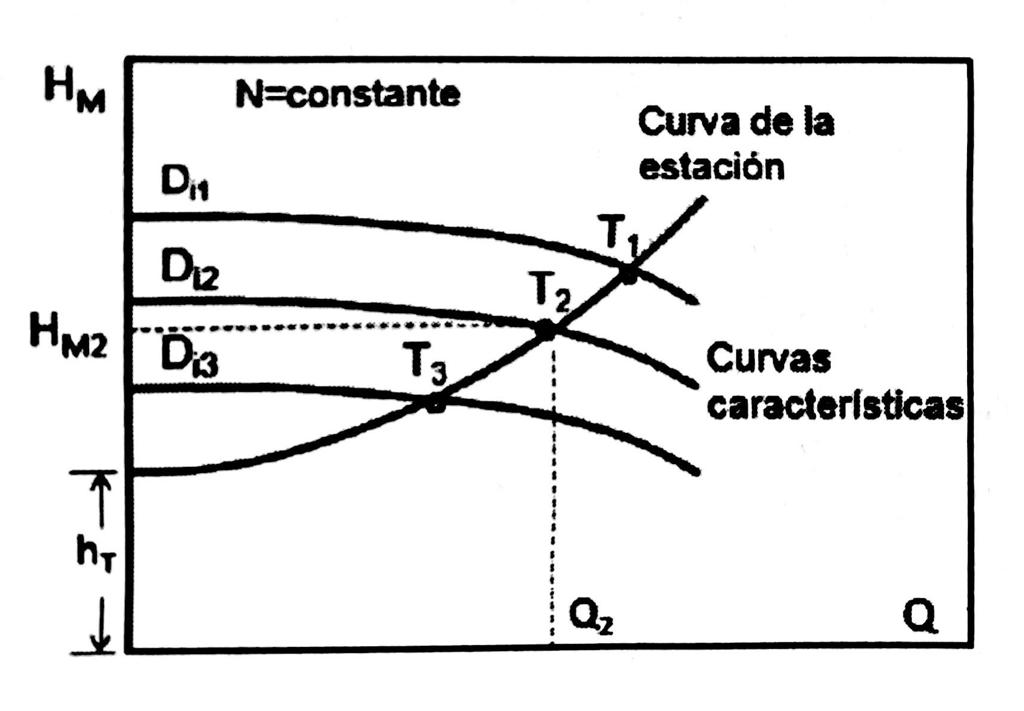
\includegraphics[width=12cm]{./figs/bom14.jpeg}
\caption{Punto de operaci\'on (tomado de \cite{agudelo2011mecanica}).} 
\label{bom14}
\end{figure}

De la misma manera, si se dibuja la curva del sistema en el gr\'afico de curva caracter\'istica de la bomba para un impulsor fijo y varios valores de $\omega$, la intersecci\'on de dichas curvas determina los puntos de  operaci\'on para diferentes valores de  $\omega$. La idea es determinar un impulsor y una velocidad de rotaci\'on que permitan proporcionar un caudal y una cabeza de energ\'ia bajo unas condiciones de alta eficiencia. Si por ejemplo el sistema requiere suministrar un  $Q_2$ y una $h_{m_2}$, el impulsor seleccionado ser\'ia $D_{i_2}$ con una velocidad de rotaci\'on $\omega$. El punto $T_2$ seria el \emph{punto de operaci\'on} o \emph{punto de trabajo} del sistema en el cual la bomba debe operar en lo posible (ver figura~\ref{bom14}). 

El punto de operaci\'on puede cambiar debido a lo siguiente (ver figura~\ref{bom15}):
\begin{itemize}
\item Variaci\'on del di\'ametro del impulsor ($D_i$) para una velocidad constante $\omega$. Si se reemplaza el impulsor por otro diferente, el punto de operaci\'on ser\'a otro.
\item Variaci\'on de la velocidad de rotaci\'on ($\omega$) para un impulsor fijo. Si $\omega$ aumenta o disminuye, el punto de operaci\'on cambiar\'a. 
\item Por variaci\'on de las perdida de energ\'ia en el sistema. Si se cambia la tuber\'ia y se colocan m\'as accesorios esto implica cambios en la perdida de energ\'ia y por tando en la curva del sistema. Por lo tanto el punto de operaci\'on cambiar\'a. 
\item Por envejecimiento de la bomba, tuber\'ias y accesorios. Con el paso del tiempo la rugosidad de las tuber\'ias aumenta as\'i como los coeficientes de perdidas de los accesorios. La bomba sufre cambios en su eficiencia y en su capacidad.  
\end{itemize}

% Duarte F8.5
\begin{figure}[h]
\centering
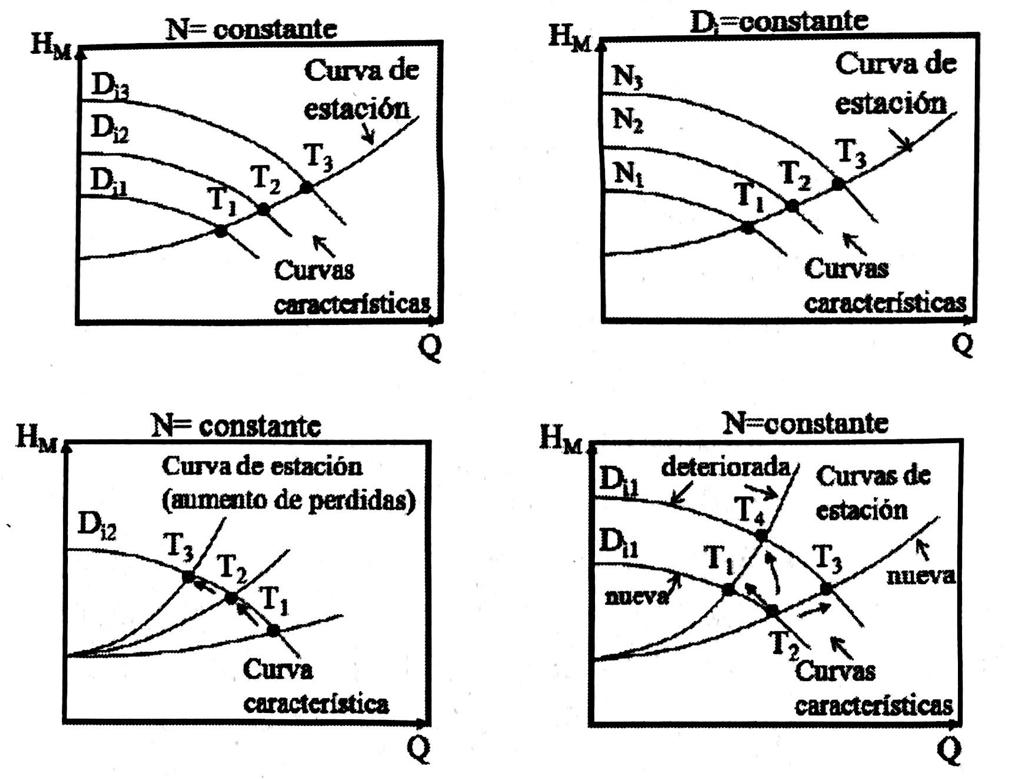
\includegraphics[width=12cm]{./figs/bom15.jpeg}
\caption{Ejemplos de variaci\'on del punto de operaci\'on (tomado de \cite{agudelo2011mecanica}).} 
\label{bom15}
\end{figure}

\subsection{Cavitaci\'on en bombas centrifugas}
La cavitaci\'on es un fen\'omeno en el cual la presi\'on est\'atica del liquido se reduce por debajo de la presi\'on de vapor del liquido (presi\'on a la cual el l\'iquido se evapora) llevando a la formaci\'on de burbujas dentro del liquido en la superficie de contacto, las cuales al desplazarse a zonas de mayor presi\'on dentro del l\'iquido explotan causando la erosi\'on de la superficie de contacto.

Para el caso de bombas centrifugas, la zona en donde es posible el desarrollo de cavitaci\'on es en la zona de acople de la tuber\'ia de succi\'on y la entrada a la bomba (ver figura~\ref{bom17}). En la zona entre la brida de la tuber\'ia de succi\'on y la carcasa de la bomba, debido a la reducci\'on gradual del di\'ametro, las velocidades del flujo aumentan y como consecuencia las presiones disminuyen considerablemente llegando al punto mas bajo de presi\'on cuando el flujo entra a la carcaza. Justo en la entrada de la carcasa, si las presiones del flujo est\'an por debajo de la presi\'on de vapor del fluido, se forman cavidades de aire que viajan a trav\'es de los alabes del impulsor a zonas de mayor presi\'on (baja velocidad) (ver figura~\ref{bom16})  causando el rompimiento de estas cavidades y la erosi\'on de los alabes (ver figura~\ref{bom16a}). Esto genera entonces una reducci\'on en la eficiencia de la bomba y problemas en la operaci\'on del sistema.

% Duarte F8.6
\begin{figure}[h]
\centering
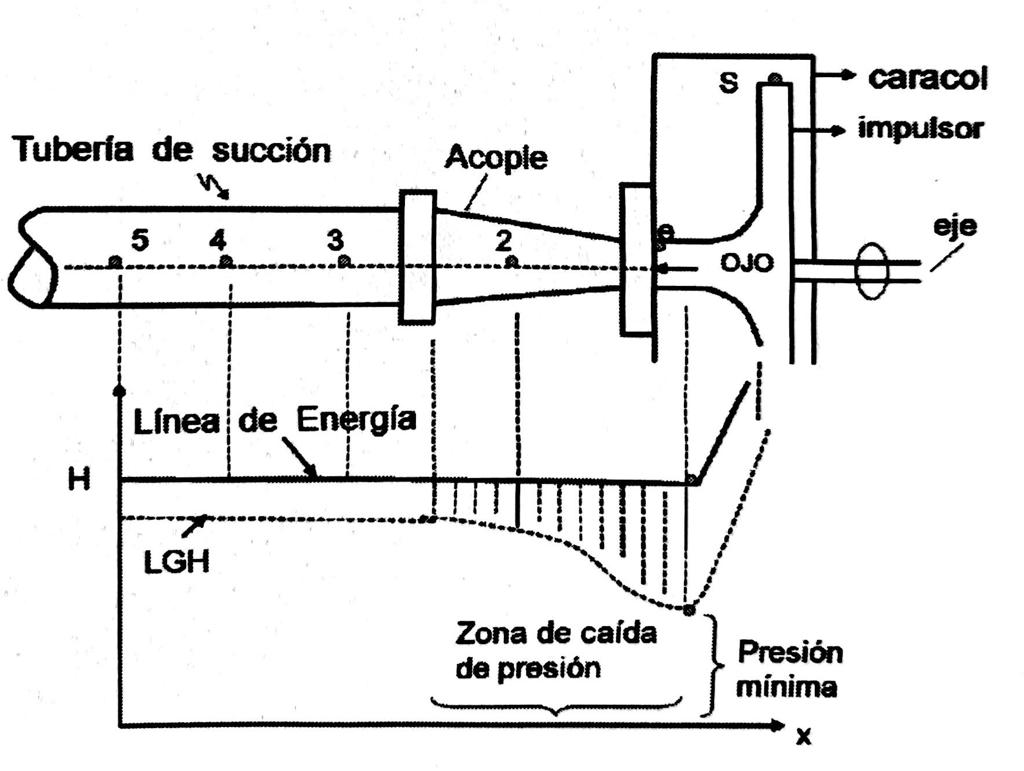
\includegraphics[width=12cm]{./figs/bom17.jpeg}
\caption{Cavitaci\'on en bombas centrifugas (tomado de \cite{agudelo2011mecanica}).} 
\label{bom17}
\end{figure}

% Inter
\begin{figure}[h]
\centering
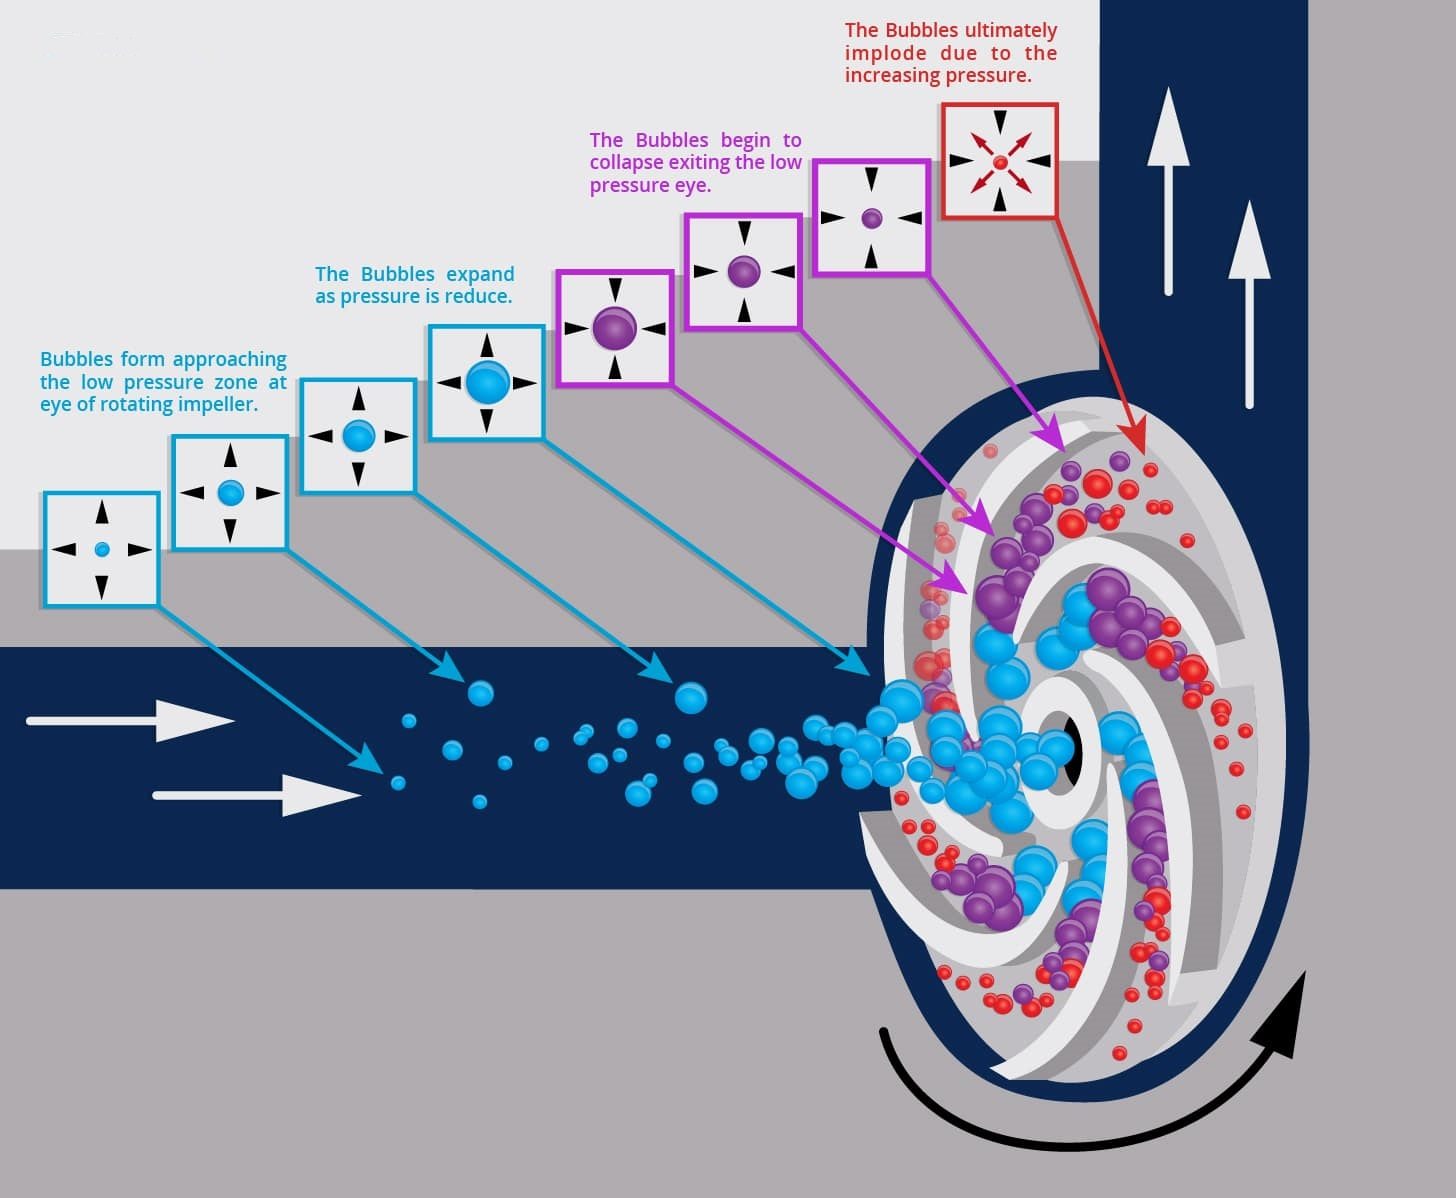
\includegraphics[width=12cm]{./figs/bom16.jpg}
\caption{Formaci\'on de cavidades de aire y explosi\'on de las mismas.} 
\label{bom16}
\end{figure}

% Inter
\begin{figure}[h]
\centering
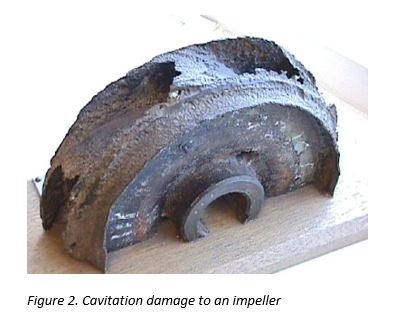
\includegraphics[width=12cm]{./figs/bom16a.JPG}
\caption{Da\~nos en el impulsor de una bomba centrifuga.} 
\label{bom16a}
\end{figure}

\subsubsection*{An\'alisis de la succi\'on}
Considerando los sistemas de succi\'on de los esquemas mostrados en la figura~\ref{bom18} y aplicando la ecuaci\'on de Bernoulli entre la superficie libre en el tanque de succi\'on y la brida de succi\'on (BS) tomando como referencia el plano de bombeo, la cabeza presi\'on en esta brida queda defina como:

% Duarte F8.8
\begin{figure}[h]
\centering
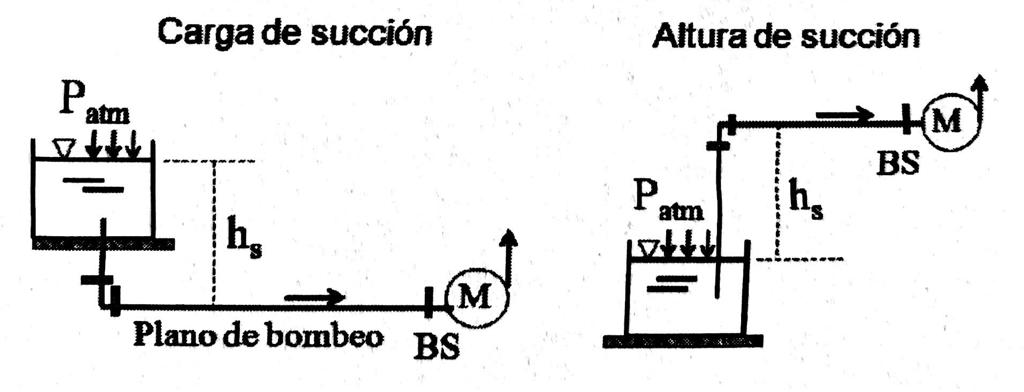
\includegraphics[width=12cm]{./figs/bom12.jpeg}
\caption{Sistemas de succi\'on en bombas centrifugas (tomado de \cite{agudelo2011mecanica}).} 
\label{bom18}
\end{figure}

\begin{equation}
\frac{P_{atm}}{\gamma} \pm h_S = \frac{P_{BS}}{\gamma} + \frac{V_{BS}^2}{2g} + \sum \left(h_f + h_e \right)
\label{boma17}
\end{equation}

despejando $\frac{P_{BS}}{\gamma}$ y dejando el termino de perdidas como una funci\'on de $Q$, se tiene:

\begin{equation}
\color{red}\boxed{\color{black} \frac{P_{BS}}{\gamma} = \frac{P_{atm}}{\gamma} \pm h_S - \frac{V_{BS}^2}{2g} - C_S Q^2 }
\label{boma18}
\end{equation}

donde $C_S$ se puede entender como un coeficiente de perdidas en la succi\'on. Analizando la ecuaci\'on~\ref{boma18}, la presi\'on en la brida de succi\'on ($P_{BS}$) disminuye si:
\begin{itemize}
\item las perdidas de energ\'ia aumentan debido a un aumento del caudal, a una gran longitud de la tuber\'ia de succi\'on, numero considerable de accesorios, tuber\'ias con material muy rugoso, tuber\'ia de succi\'on dise\~nada con di\'ametro peque\~no.
\item de acuerdo con la posici\'on del tanque de succi\'on, si aumenta o disminuye la altura est\'atica de la succi\'on.
\item si se disminuye la presi\'on atmosf\'erica  local, por ejemplo, cuando el proyecto se desarrolla en lugares elevados con respecto al nivel del mar. 
\item si aumenta la presi\'on de vapor del fluido lo cual implica que la probabilidad de que ocurra cavitaci\'on aumente. 
\item si el impulsor rota a una velocidad mayor a la recomendada por el fabricante. Esto implica que las cavidades viajen y exploten m\'as r\'apidamente en este.  
\end{itemize}

Para evitar que se presente cavitaci\'on por las razones antes mencionadas, es necesario determinar una cabeza neta m\'inima.

\subsubsection*{Cabeza neta de succi\'on positiva disponible ($NPSH_D$)}
La cabeza neta de succi\'on positiva disponible ($NPSH_D$) se define como la energ\'ia absoluta en la brida de succi\'on con respecto al plano de bombeo menos la cabeza de presi\'on de vapor del fluido que circula por el sistema. De acuerdo con lo anterior y con base en la ecuaci\'on~\ref{boma17} se puede decir que la energ\'ia absoluta en la brida de succi\'on ($h_{sa}$), se puede expresar como:

\begin{equation}
h_{sa} = \frac{P_{atm}}{\gamma} \pm h_S - C_S Q^2 = \frac{P_{BS}}{\gamma} + \frac{V_{BS}^2}{2g} 
\label{boma19}
\end{equation}

Si a $h_{sa}$ le restamos la cabeza de presi\'on de vapor del liquido del sistema, se tiene que $NPSH_D$:

\begin{equation}
\color{red}\boxed{\color{black} NPSH_D = h_{sa} -\frac{P_v}{\gamma} = \frac{P_{atm}}{\gamma} \pm h_S - C_S Q^2 -\frac{P_v}{\gamma} = \frac{P_{BS}}{\gamma} + \frac{V_{BS}^2}{2g} -\frac{P_v}{\gamma}}
\label{boma19}
\end{equation}


\subsubsection*{$NPSH$ requerido}
La cabeza neta de succi\'on positiva requerida  $NPSH_R$ se determina mediante ensayos de laboratorio en donde en una bomba centrifuga para una velocidad $\omega$ y caudal constante se varia la $NPSH_D$ y se determina los valores de la carga o altura neta $h_m$. Se supone que $h_m$ es constante para cualquier valor de $NPSH_D$, sin embargo, esto no es as\'i por lo cual al graficar los datos de $NPSH_D$ vs $h_m$ se observa una ca\'ida de $h_m$ cuando $NPSH_D$ disminuye (ver figura~\ref{bom19}). De acuerdo con esto, $NPSH_R$ es igual a $NPSH_D$ para el cual el valor de $h_m$ disminuye en un 3\%, lo que indica que a partir de este valor inicia la cavitaci\'on

% Duarte F8.10
\begin{figure}[h]
\centering
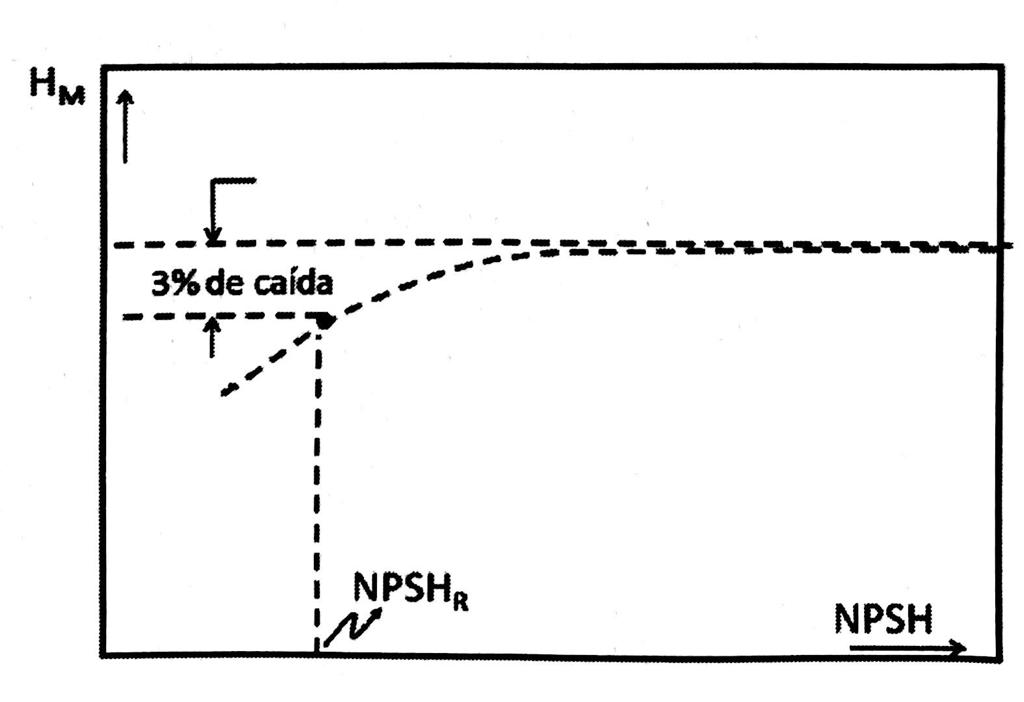
\includegraphics[width=12cm]{./figs/bom19.jpeg}
\caption{Determinaci\'on de $NPSH_R$ (tomado de \cite{agudelo2011mecanica}).} 
\label{bom19}
\end{figure}

Si se varia el caudal en la bomba, se puede obtener una curva de $NPSH_R$ vs $Q$ como la que se muestra en la figura~\ref{bom20}. Dicha curva muestra un aumento de $NPSH_R$ con el aumento de $Q$ lo cual se da porque al aumentar $Q$ disminuye $h_m$ y la ca\'ida de $h_m$ se anticipa resultando en mayores valores de $NPSH_R$.  

% Duarte F8.11
\begin{figure}[h]
\centering
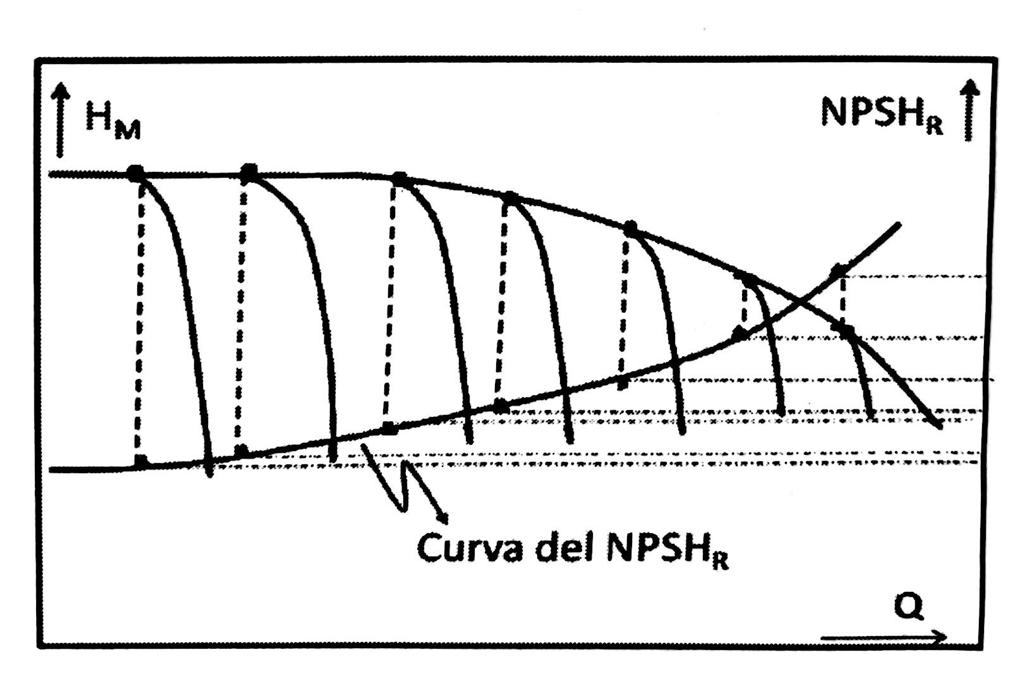
\includegraphics[width=12cm]{./figs/bom20.jpeg}
\caption{Curva de $NPSH_R$ vs $Q$ (tomado de \cite{agudelo2011mecanica}).} 
\label{bom20}
\end{figure}

Al analizar la ecuaci\'on~\ref{boma19}, se observa que $NPSH_D$ disminuye con el aumento del caudal $Q$ mientras que, de acuerdo con la figura~\ref{bom20}, $NPSH_R$ aumenta con el aumento de $Q$. La figura~\ref{bom21}  muestra la variaci\'on de $NPSH_D$ y de $NPSH_R$ como una funci\'on del caudal, y se observa que el punto de corte de las dos curvas (P) define la ocurrencia incipiente de cavitaci\'on. Por lo tanto, para el dise\~no del sistema de succi\'on es necesario que $NPSH_D > NPSH_R$. Gracias a la practica, se recomienda que $NPSH_D > 1.35 NPSH_R$

% Duarte F8.12
\begin{figure}[h]
\centering
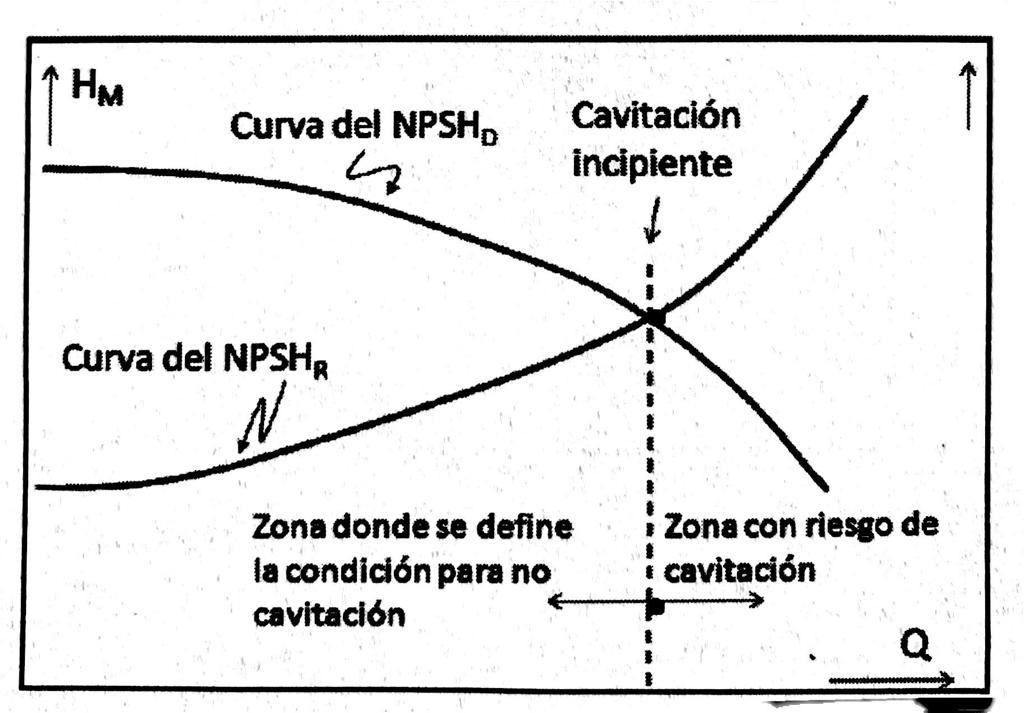
\includegraphics[width=12cm]{./figs/bom21.jpeg}
\caption{Condici\'on para evitar la cavitaci\'on (tomado de \cite{agudelo2011mecanica}).} 
\label{bom21}
\end{figure}

\subsubsection*{Par\'ametro de cavitaci\'on}
De acuerdo con el an\'alisis dimensional de sistemas de bombeo para un di\'ametro $D_i$ constante, tenemos que los par\'ametros adimensionales son:

\begin{equation}
\Pi_1 = \frac{Q}{\omega D_i^3} = \frac{Q}{\omega} \quad Q \propto \omega  \quad \quad \Pi_2 = \frac{g h_m}{\omega^2 D_i^2} = \frac{h_m}{\omega^2} \quad h_m \propto \omega^2
\label{boma20}
\end{equation}

Analizando la relaci\'on de $NPSH_R$ vs $Q$ se puede decir que $NPSH_R \propto Q^2$ y de acuerdo con las relaciones de la ecuaci\'on~\ref{boma20}, tenemos que $NPSH_R \propto h_m$. Por lo tanto, se puede crear un par\'ametro adimensional, conocido como el \emph{parametro de cavitaci\'on} ($\sigma$) igual a:

\begin{equation}
\color{red}\boxed{\color{black} \sigma = \frac{NPSH_R}{h_m} }
\label{boma21}
\end{equation}


\subsubsection*{Velocidad espec\'ifica de succi\'on}
En la modelaci\'on f\'isica en hidr\'aulica, es frecuente utilizar un par\'ametro conocido como la \emph{velocidad espec\'ifica de succi\'on} ($S_S$). Si se reemplaza $h_m$ en la ecuaci\'on~\ref{boma14} de la velocidad espec\'ifica por $NPSH_R$, se tiene:

\begin{equation}
S_S = \frac{\omega \sqrt{Q}}{NPSH_R^{3/4}}
\label{boma22}
\end{equation}

Utilizando la ecuaci\'on~\ref{boma22} y la ecuaci\'on~\ref{boma14}, se tiene que el siguiente par\'ametro (\emph{p\'arametro de Thomas}):

\begin{equation}
\sigma_C = \frac{NPSH_R}{h_m} = \left(\frac{n_S}{S_S} \right)^{4/3}
\label{boma23}
\end{equation}

La ecuaci\'on anterior indica que para un valor dado de $n_S$, valores bajos de $S_S$ indican que la bomba tiene un margen de seguridad m\'as alto. Ademas cuando bombas de una misma serie homologa operan bajo condiciones de cavitaci\'on, valores iguales de $S_S$ indican un grado de cavitaci\'on  semejante. Se ha podido demostrar que para bombas de succi\'on simple, $\sigma_C$ se convierte en:

\begin{equation}
\sigma_C =  \frac{\phi n_S^{4/3}}{10^6} 
\label{boma24}
\end{equation}

en donde $\phi = 1210$ para sistema internacional ($Q$ en $m^3/s$ y $h_m$ $m$). Para bombas de succi\'on doble, se tiene:

\begin{equation}
\sigma_C =  \frac{4 n_S^{4/3}}{10^6} 
\label{boma25}
\end{equation}

la cual es valida para sistema ingles de unidades ($Q$ in $gpm$ y $h_m$ en $pies$).

\subsection{Sistemas con bombas en serie}
Los sistemas de bombas en serie se utilizan en sistemas de tuber\'ias cuando la carga est\'atica a vencer es muy alta tal que se requiere m\'as de una bomba para suministrar esta energ\'ia. Para esto, se disponen bombas una detr\'as de otra, en donde para las bombas siguientes a la primera, la tuber\'ia de succi\'on de la bomba siguiente es la tuber\'ia de descarga de la bomba inmediatamente anterior (ver figura~\ref{bom22}). Por lo tanto, la carga total suministrada por las bombas para un caudal dado, es la suma de las cargas suministradas por las bombas.

% Duarte F8.17
\begin{figure}[h]
\centering
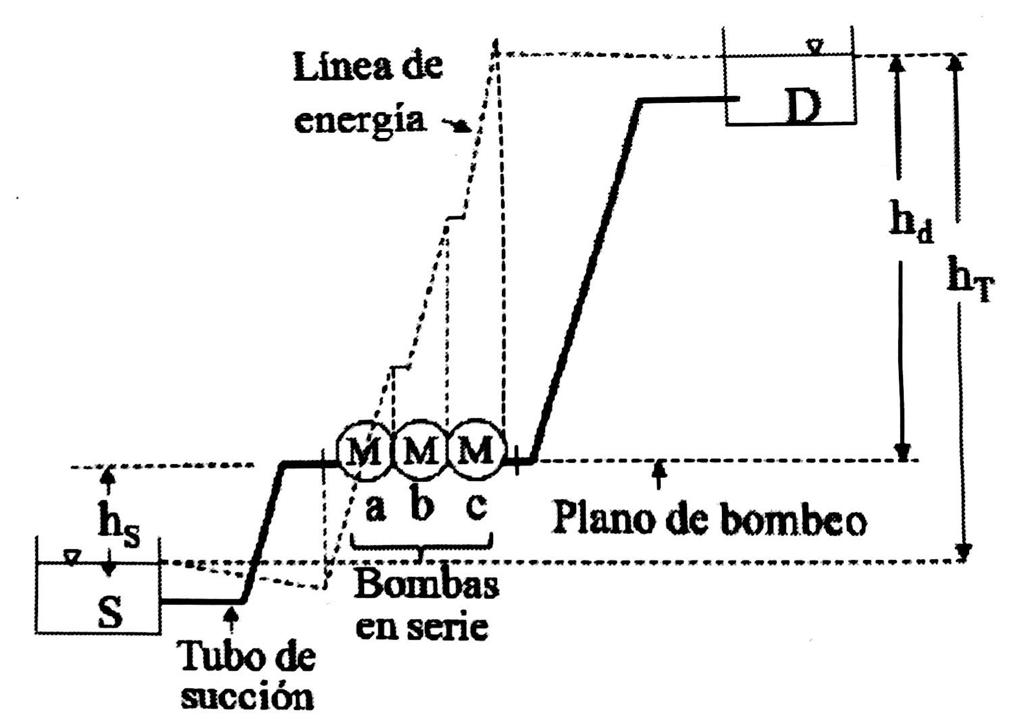
\includegraphics[width=12cm]{./figs/bom22.jpeg}
\caption{Sistema de bombas en serie (tomado de \cite{agudelo2011mecanica}).} 
\label{bom22}
\end{figure}

Si se supone que se tiene un sistema de dos  bombas (a y b) centrifugas en serie, el punto de operaci\'on de un sistema de bombas en serie se define mediante las curvas caracter\'isticas de las bombas individuales y la combinaci\'on de ambas (ver figura~\ref{bom23}). Para un caudal $Q_i$ que transporta el sistema, los valores de la carga para la bomba a y b son $h_{m_a}$ y $h_{m_b}$, respectivamente, mientras que la carga que suministran ambas bombas para $Q_i$ es la suma aritm\'etica $h_{m_a}+h_{m_b}$. La curva caracter\'istica del sistema de dos bombas en serie se puede obtener mediante la suma de las $h_m$ para diferentes caudales. De acuerdo con esto, el punto de operaci\'on del sistema (punto T) es entonces el corte de la curva del sistema  o curva de la estaci\'on (curva E) con la curva caracter\'istica del sistema en serie.  

% Duarte F8.18
\begin{figure}[h]
\centering
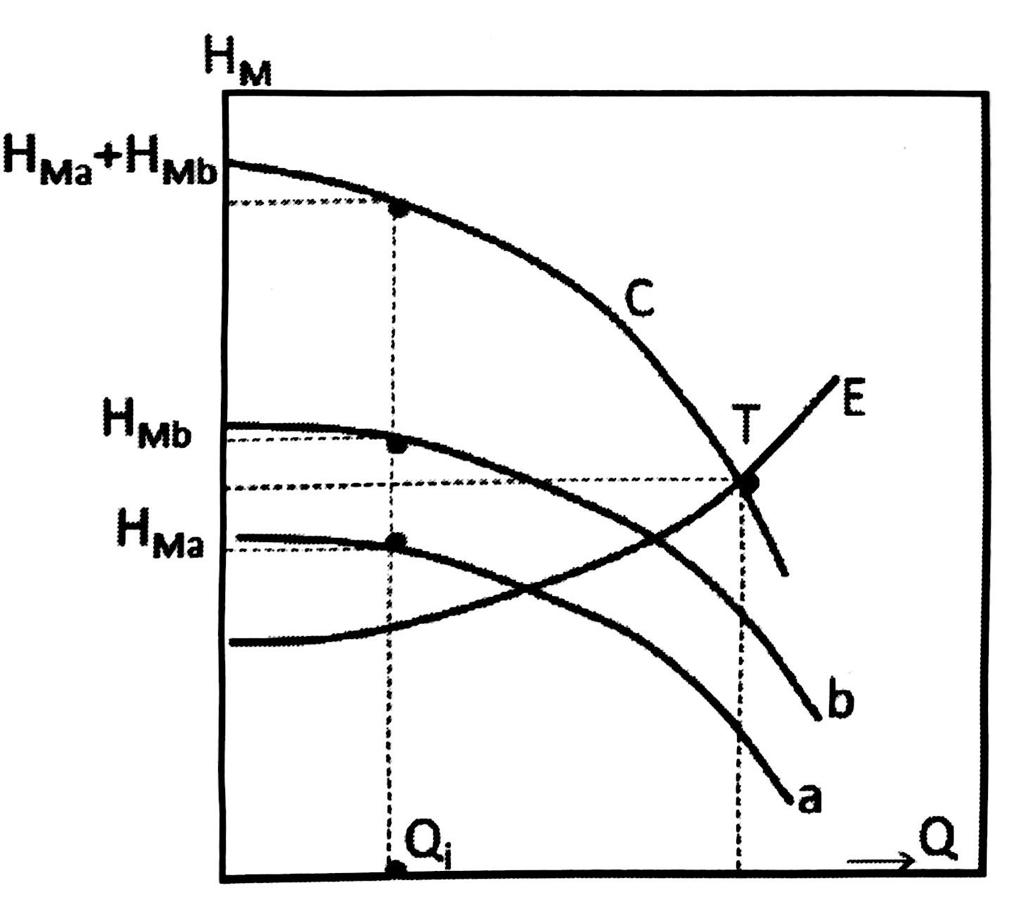
\includegraphics[width=12cm]{./figs/bom23.jpeg}
\caption{Punto de operaci\'on de un sistema con dos bombas en serie (tomado de \cite{agudelo2011mecanica}).} 
\label{bom23}
\end{figure}


Note que en la figura~\ref{bom23}, el punto de operaci\'on o de trabajo T corresponde a una mayor carga que las proporcionadas por cada una de las bombas, pero dicha carga es menor que la suma de las cargas (e.g. $h_{m_a}+ h_{m_b}$). La eficiencia de cada bomba queda definida por el caudal que suministra cada bomba. 


\subsection{Sistemas con bombas en paralelo}
Si se tiene un sistema de tuber\'ias en donde es necesario suministrar un caudal alto para una carga alta, es necesario la instalaci\'on de bombas en paralelo. Las bombas en paralelo suministran un caudal total, que constituye la suma de los caudales suministrados por cada bomba, para una carga determinada (ver figura~\ref{bom24}). Si se tienen dos bombas, a y b, como en la figura~\ref{bom24} cuyas curvas caracter\'isticas est\'an representadas en la figura~\ref{bom25}, la curva caracter\'istica del sistema en paralelo (curva c) se puede formar a partir de las curvas caracter\'isticas de a y b sumando los caudales ($Q_c = Q_a + Q_b$) para una misma carga $h_{m_i}= h_{m_a}=h_{m_b}$. El punto de operaci\'on o punto de trabajo del sistema es la intersecci\'on de la curva caracteristica para las dos bombas en paralelo y la curva E del sistema. La eficiencia de cada bomba depende del caudal que suministra cada una de ellas. 

% Duarte F8.24
\begin{figure}[h]
\centering
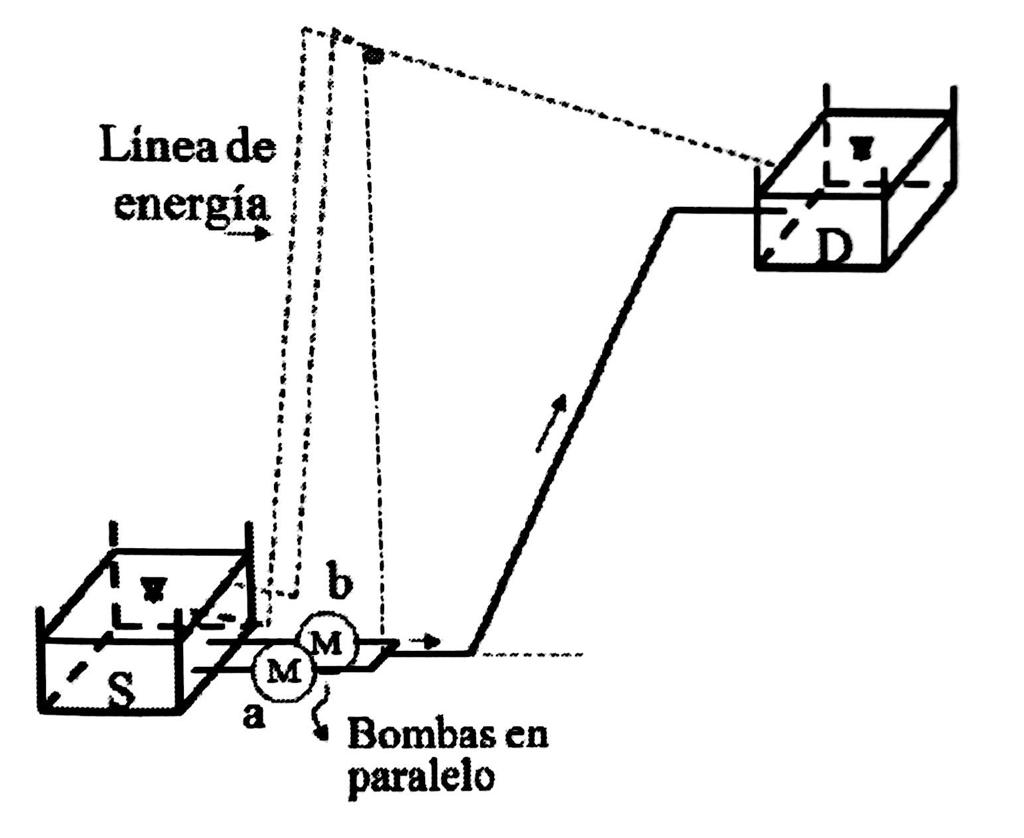
\includegraphics[width=12cm]{./figs/bom24.jpeg}
\caption{Sistema de bombas en paralelo (tomado de \cite{agudelo2011mecanica}).} 
\label{bom24}
\end{figure}

% Duarte F8.25
\begin{figure}[h]
\centering
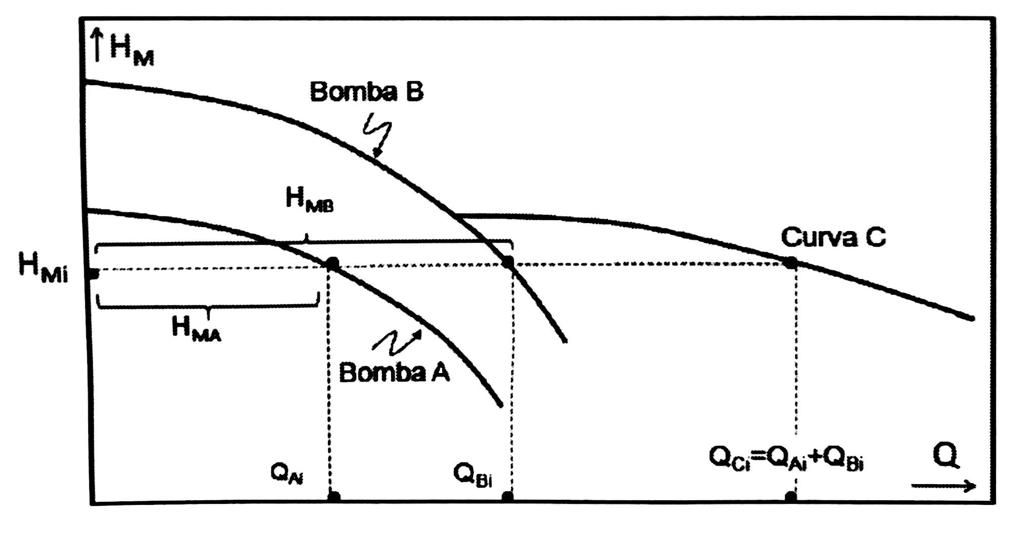
\includegraphics[width=12cm]{./figs/bom25.jpeg}
\caption{Curva caracter\'istica de dos bombas en paralelo (tomado de \cite{agudelo2011mecanica}).} 
\label{bom25}
\end{figure}


\subsection{Sistemas especiales}



% REFERENCES
\bibliographystyle{plain} % We choose the "plain" reference style
\bibliography{refs} % Entries are in the refs.bib file



\end{document}
